\documentclass[a3paper,14pt]{extarticle}
\usepackage{extsizes}
\usepackage{cmap}
\usepackage[utf8]{inputenc}
\usepackage[T2A]{fontenc}
\usepackage[english,russian]{babel} 
\usepackage[left=15mm, top=25mm, right=15mm, bottom=30mm, nohead, nofoot]{geometry}
\usepackage{graphicx}  % изобржаения
\usepackage{wrapfig}  % изобржаения
\usepackage{tikz} % графика
\usepackage{xcolor} % определение цветов
\usepackage{nicefrac} % красивые дроби
\usepackage{cancel} % сокращение
\usepackage{amsmath,amsfonts,amssymb} % математический пакет
\usepackage{fancybox,fancyhdr} % хедер и футер
\pagestyle{fancy}
\fancyhf{}
\fancyhead[L]{Практическая линейная алгебра}
\fancyhead[R]{Овчинников Павел}
\fancyfoot[C]{\thepage}
\setcounter{page}{1}
\headsep=10mm
\footskip=15mm
\usepackage{hyperref}  % гиперссылки

\definecolor{urlcolor}{HTML}{3454D1}

\hypersetup{pdfstartview=FitH, linkcolor=linkcolor,urlcolor=urlcolor, colorlinks=true}

\newlength{\tempheight}
\newcommand{\Let}{
\mathbin{\text{\settoheight{\tempheight}{\mathstrut}\raisebox{0.4\pgflinewidth}{
\tikz[baseline=0.5ex,line cap=round,line join=round] \draw (0,0) --++ (0.3em,0) --++ (0,2.3ex) --++ (-0.3em,0);
}}}}
\newcommand*\squared[1]{\tikz[baseline=(char.base)]{
            \node[shape=rectangle,draw,inner sep=4pt] (char) {$#1$};}}
\newcommand{\at}{\biggr\rvert}
\newcommand{\shiftright}[3]{\makebox[#2][r]{\makebox[#1][l]{#3}}}

\newcommand\NB{\textbf{N\kern-0.32em\textcolor{red}{B}}}
\newcommand{\observ}[1]{\textbf{\textit{Рубрика «наблюдения»}:} \textit{#1}}

\begin{document}
\section*{\centering Лабораторная работа №4}
\subsection*{\centering Задание №1. Снова Imagine Dragons?}
Зададим два неколлинеарных вектора $\hat{v}_1 = \left[\begin{smallmatrix}
    1 \\ 2
\end{smallmatrix}\right]$ и $\hat{v}_2 = \left[\begin{smallmatrix}
    1 \\ -1
\end{smallmatrix}\right]$, которые будем использовать в задании для получения динамических систем. Для удобства я накрыл их крышечками, чтобы мы не путали их с собственными векторами :)
\subsubsection*{Пункт №1}
Система асимптотически устойчива, когда собственные числа матрицы $\lambda < 0$. Теперь рассмотрим решение системы $x(t) = e^{At}x(0)$: заметим, что если $x(t) \in \text{Span}\{\hat{v}_1\} \cup \text{Span}\{\hat{v}_2\}$ для каждого из условий $x(0) = \hat{v}_1 \cup \hat{v}_2$ соответственно, то тогда можно прийти к выводу, что решение такой системы выглядит как $\alpha x(0) = e^{At}x(0)\ \Rightarrow\ \alpha E = e^{At}$ ($E$ --- единичная матрица), соблюдая константно-матричное соотношение. Получается, нам достаточно задать матрицу $A$ как матрицу с любыми отрицательными числами на главной диагонали:
$$A = \begin{bmatrix}
    -2 & 0 \\ 0 & -2
\end{bmatrix}$$
Нетрудно отсюда понять, что собственное число матрицы $\lambda_1 = -2$, собственных векторов два $v_1=\left[\begin{smallmatrix}
    1 \\ 0
\end{smallmatrix}\right], v_2= \left[\begin{smallmatrix}
    0 \\ 1
\end{smallmatrix}\right]$, т.к. пространство масштабируется под действием матрицы $A$.
\subsubsection*{Пункт №2}
Система неустойчива, когда собственные числа матрицы $\lambda > 0$. Формальное объяснение, как получить матрицу, у которой не существует двух неколлинеарных собственных векторов, будет очень развёрнутым (представлено в пункте №4), поэтому я просто покажу пример такой матрицы и найду её собственное число, собственный вектор и обобщённый собственный вектор.
$$A = \begin{bmatrix}
    1 & 0 \\ 1 & 1
\end{bmatrix}$$
Собственное число $\lambda = 1$, собственный вектор $v_1 = \left[\begin{smallmatrix}
    0 \\ 1
\end{smallmatrix}\right]$, присоединённый к $v_1$ вектор $u_1 = \left[\begin{smallmatrix}
    1 \\ 0
\end{smallmatrix}\right]$.
\subsubsection*{Пункт №3}
С ростом $t$ вектор $\hat{v}_1$ должен сжиматься в $\left[\begin{smallmatrix}
    0 \\ 0
\end{smallmatrix}\right]$, но т.к. система неустойчива, то нам жизненно необходимо наращивать вектор $\hat{v}_2$ с ростом $t$... Да-да, вы понимаете, о чём я, нам снова придётся решать те системки с лабораторной работы №2 --- въетнамские флешбеки, получается:
$$\begin{bmatrix}
    x_1 & x_2 \\ x_3 & x_4
\end{bmatrix}\begin{bmatrix}
    1 \\ 2
\end{bmatrix} = \begin{bmatrix}
    0 \\ 0
\end{bmatrix} \  \Rightarrow \ \begin{cases}
    x_1 + 2x_2 = 0 \\ x_3 + 2x_4 = 0
\end{cases}$$
$$\begin{bmatrix}
    x_1 & x_2 \\ x_3 & x_4
\end{bmatrix}\begin{bmatrix}
    1 \\ -1
\end{bmatrix} = \begin{bmatrix}
    2 \\ -2
\end{bmatrix} \ \Rightarrow \ \begin{cases}
    x_1 - x_2 = 2 \\ x_3 - x_4 = -2
\end{cases}$$
Скомпонуем системы так, чтобы в одной системе были только $x_1$ и $x_2$, а в другой в то же время $x_3$ и $x_4$:
$$\begin{cases}
    x_1 + 2x_2 = 0 \\ x_1 - x_2 = 2
\end{cases} \Rightarrow\ \begin{cases}
    x_1 = 2 + x_2 \\ 3x_2 = -2
\end{cases} \Rightarrow\ \begin{cases}
    x_1 = 2 + x_2 \\ x_2 = \nicefrac{-2}{3}
\end{cases} \Rightarrow\ \begin{cases}
    x_1 = \nicefrac{4}{3} \\ x_2 = \nicefrac{-2}{3}
\end{cases}$$
$$\begin{cases}
    x_3 + 2x_4 = 0 \\ x_3 - x_4 = -2
\end{cases} \Rightarrow\ \begin{cases}
    x_3 = x_4 -2 \\ 3x_4 = 2
\end{cases} \Rightarrow\ \begin{cases}
    x_3 = x_4 - 2 \\ x_4 = \nicefrac{2}{3}
\end{cases} \Rightarrow\ \begin{cases}
    x_3 = \nicefrac{-4}{3} \\ x_4 = \nicefrac{2}{3}
\end{cases}$$
И получаем итоговую матрицу $A$:
$$A = \begin{bmatrix}
    \nicefrac{4}{3} & \nicefrac{-2}{3} \\ \nicefrac{-4}{3} & \nicefrac{2}{3}
\end{bmatrix}$$
Собственные числа этой матрицы $\lambda_1 = 0$ и $\lambda_2 = 2$, а собственные вектора, соответствующие собственным числам $v_1 = \left[\begin{smallmatrix}
    1 \\ 2
\end{smallmatrix}\right]$ и $v_2 = \left[\begin{smallmatrix}
    -1 \\ 1
\end{smallmatrix}\right]$. \\[0.5em]
\observ{заметим, что собственные вектора совпадают с выбранными $\hat{v}_1$ и $\hat{v}_2$ --- действительно, сама матрица работает именно с этими векторами, сжимая первый в ноль и увеличивая второй в 2 раза.}\pagebreak
\subsubsection*{Пункт №4}
Напомню и уточню, что система асимптотически устойчива, когда собственные числа матрицы $Re(\lambda) < 0$. Итак, мы имеем базис собственных векторов $P=\left[\begin{smallmatrix}
    1+2i & 1-2i \\ 1-i & 1+i
\end{smallmatrix}\right]$ и нам нужно только лишь подобрать диагональную матрицу собственных чисел $D$ (очевидно, они также будут комплексными), чтобы получить искомую матрицу $A \in \mathbb{R}^2$. Учитывая, что комплексные собственные числа всегда идут сопряжёнными парами, мы просто выберем рациональную часть, удовлетворяющую условию асимптотической устойчивости, а мнимую часть подберём такую, чтобы избавиться от дробей --- чисто эстетики ради:
$$A = PDP^{-1} = \begin{bmatrix}
    1+2i & 1-2i \\ 1-i & 1+i
\end{bmatrix}\begin{bmatrix}
    -1-3i & 0 \\ 0 & -1+3i
\end{bmatrix}\begin{bmatrix}
    1+2i & 1-2i \\ 1-i & 1+i
\end{bmatrix}^{-1} = \begin{bmatrix}
    0 & 5 \\ -2 & -2
\end{bmatrix}$$
Поиск собственных чисел и собственных векторов здесь не требуется --- они все указаны в разложении выше. 
\subsubsection*{Пункт №5}
Ну тут совсем уж думать не надо. Чтобы система выше стала неустойчивой при тех же собственных векторах, надо всего лишь сделать рациональную часть собственных чисел положительной.
$$A = PDP^{-1} = \begin{bmatrix}
    1+2i & 1-2i \\ 1-i & 1+i
\end{bmatrix}\begin{bmatrix}
    1-3i & 0 \\ 0 & 1+3i
\end{bmatrix}\begin{bmatrix}
    1+2i & 1-2i \\ 1-i & 1+i
\end{bmatrix}^{-1} = \begin{bmatrix}
    2 & 5 \\ -2 & 0
\end{bmatrix}$$
Собственные числа и собственные вектора я вновь не ищу, ведь они представлены в разложении выше.
\subsubsection*{Пункт №6}
Последние два пункта самые крутые! Система не асимптотически устойчива, если $Re(\lambda) = 0$. Тогда матрица будет вращать динамическую систему, а траектория будет фиксирована.
$$A = PDP^{-1} = \begin{bmatrix}
    1+2i & 1-2i \\ 1-i & 1+i
\end{bmatrix}\begin{bmatrix}
    -3i & 0 \\ 0 & 3i
\end{bmatrix}\begin{bmatrix}
    1+2i & 1-2i \\ 1-i & 1+i
\end{bmatrix}^{-1} = \begin{bmatrix}
    1 & 5 \\ -2 & -1
\end{bmatrix}$$
И снова я не указываю собственные числа и собственные вектора --- их можно увидеть выше в разложении.\\[1em]
\subsection*{\centering Задание №2. Model is on the stage}
Зададим три начальных условия $x_1(0) = \left[\begin{smallmatrix}
    8 \\ 3
\end{smallmatrix}\right]$, $x_2(0) = \left[\begin{smallmatrix}
    -5 \\ 4
\end{smallmatrix}\right]$, $x_3(0) = \left[\begin{smallmatrix}
    2 \\ -4
\end{smallmatrix}\right]$. Теперь будем:\begin{enumerate}
    \item вычислять $\left[\begin{smallmatrix}
        x_1(t) \\ x_2(t)
    \end{smallmatrix}\right]$ для каждой из систем выше, подставляя общее начальное условие $x(0) = \left[\begin{smallmatrix}
        a \\ b
    \end{smallmatrix}\right]$;
    \item заменять $a$ и $b$ на заданные выше начальные условия;
    \item визуализировать на графике траекторию движения точек с течением времени $t$.
\end{enumerate}
\subsubsection*{Пункт №1}
\begin{wrapfigure}[16]{r}{0.5\textwidth}
    \centering
    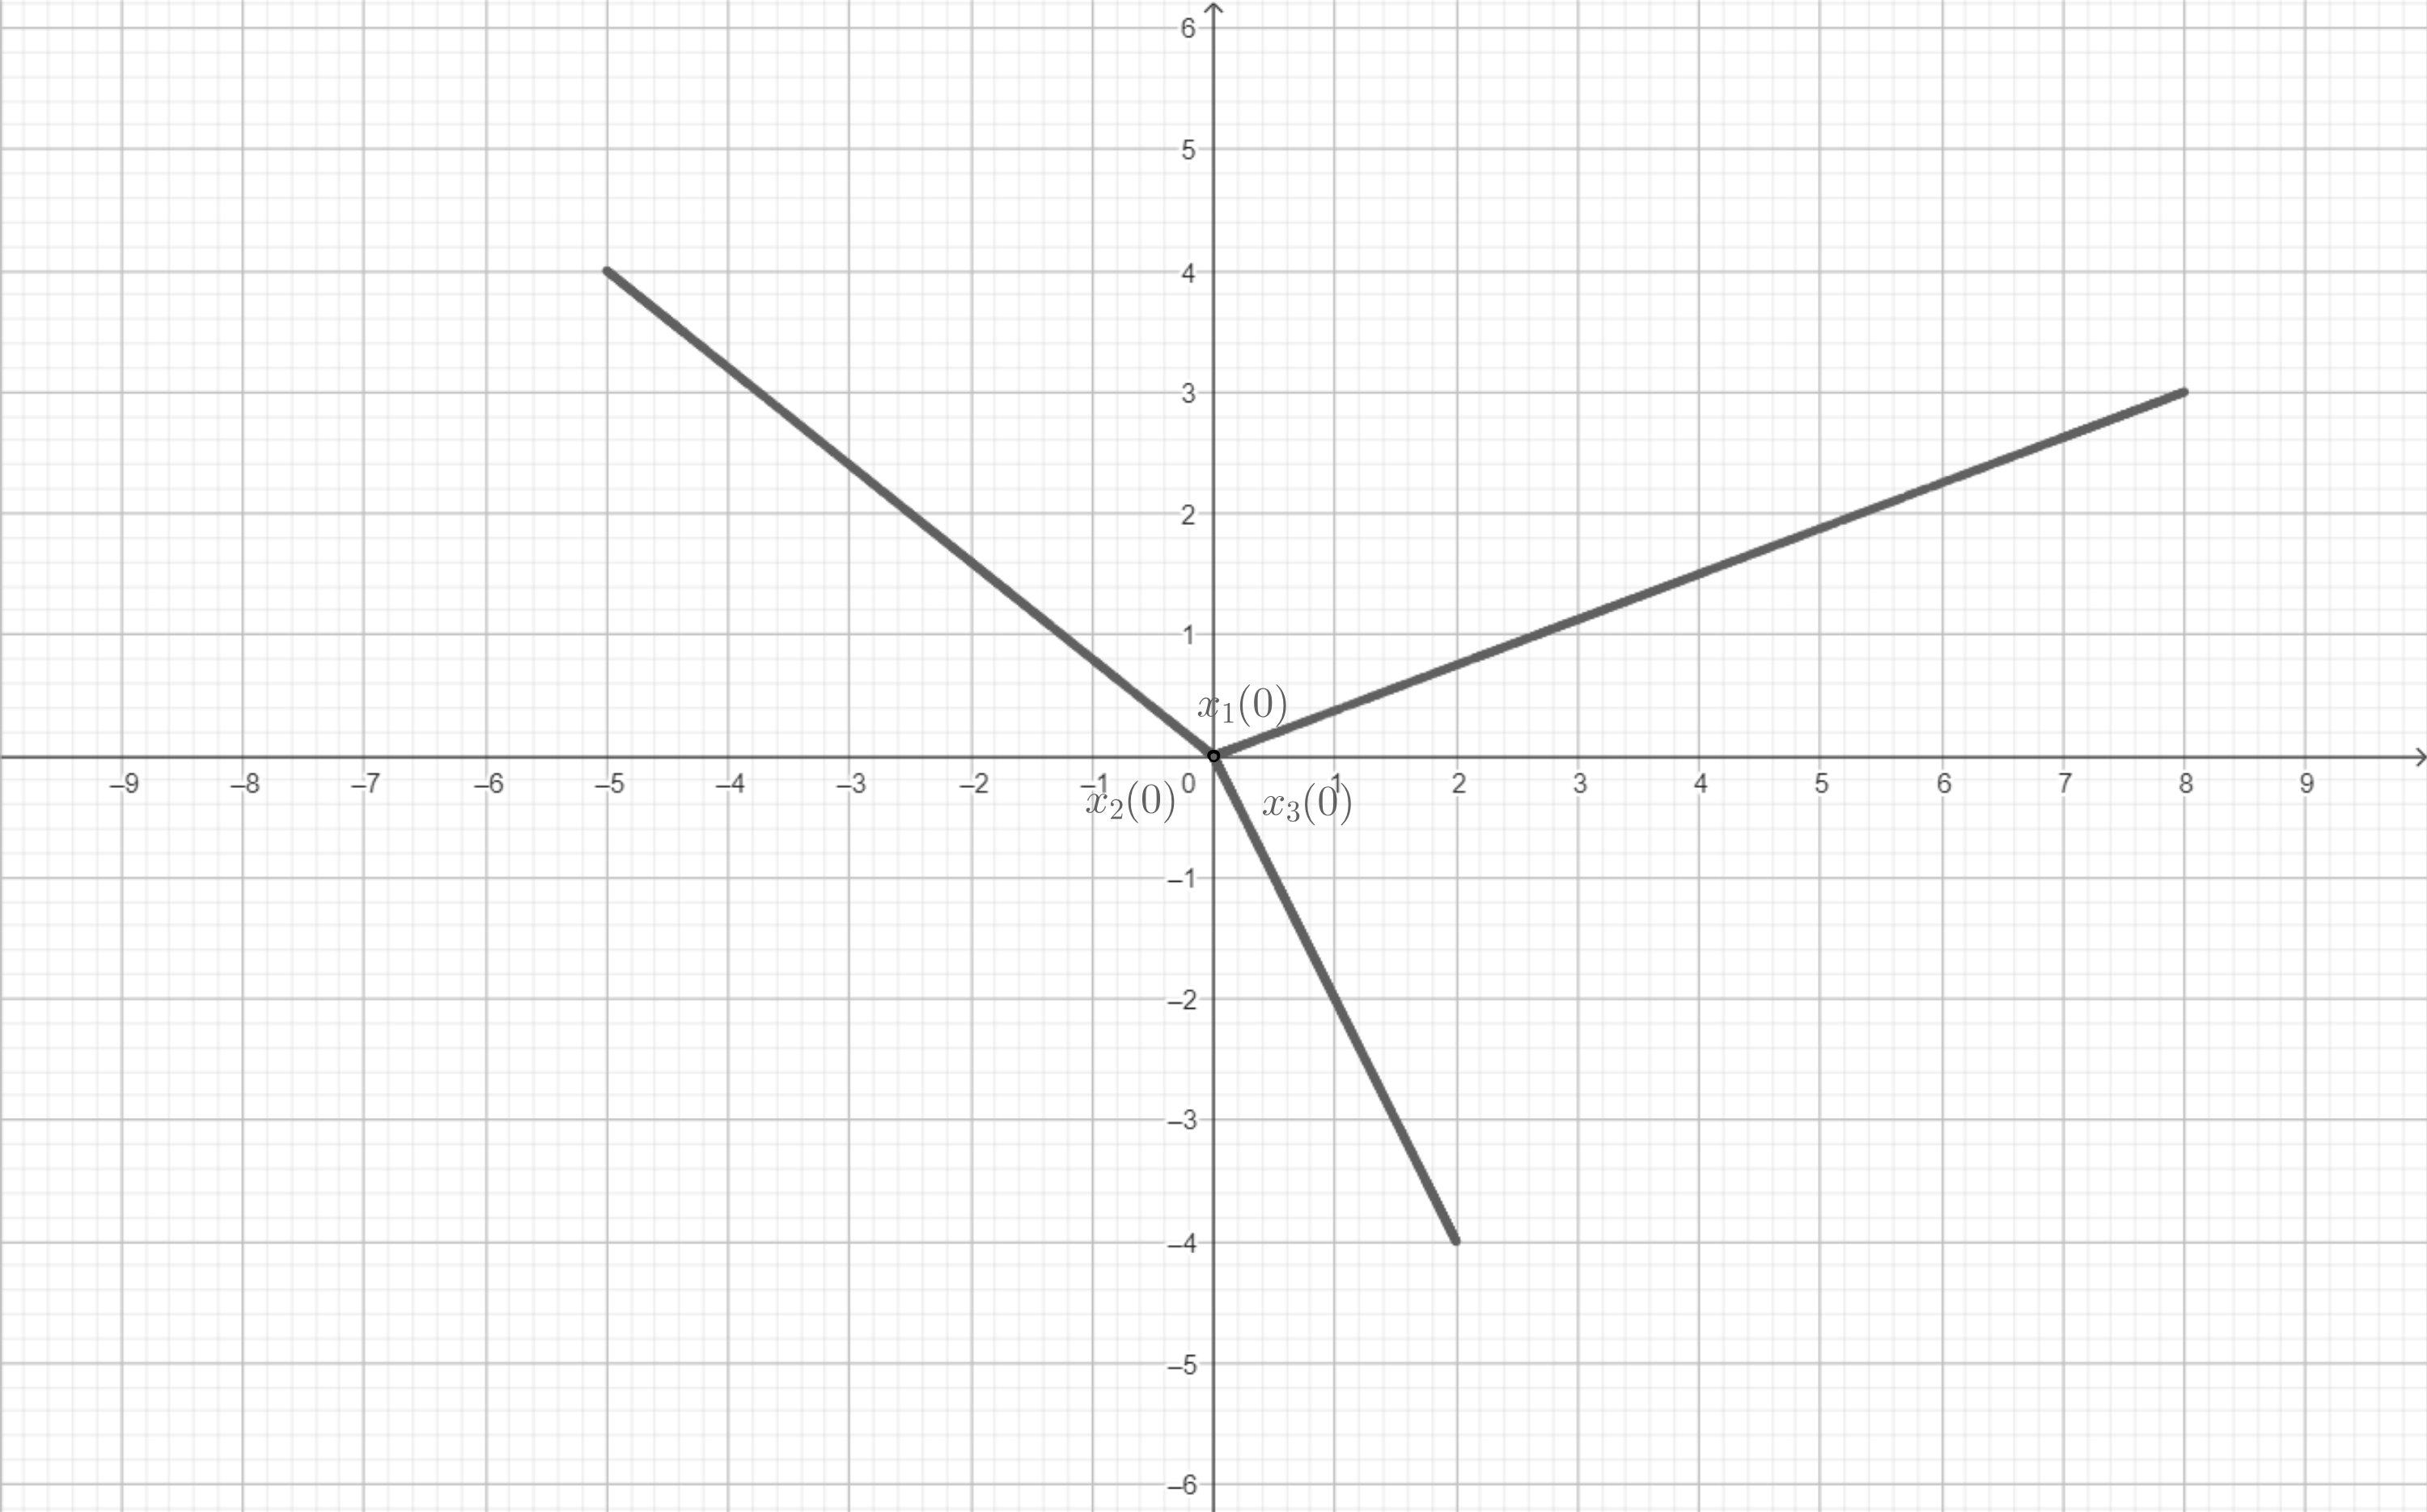
\includegraphics[width=0.5\textwidth]{2.1.png}
\end{wrapfigure}
$$\begin{bmatrix}
    x_1(t) \\ x_2(t)
\end{bmatrix} = e^{\left[\begin{smallmatrix}
    -2 & 0 \\ 0 & -2
\end{smallmatrix}\right]t}\begin{bmatrix}
    a \\ b
\end{bmatrix} = \begin{bmatrix}
    e^{-2t} & 0 \\ 0 & e^{-2t}
\end{bmatrix}\begin{bmatrix}
    a \\ b
\end{bmatrix} = \begin{bmatrix}
    \nicefrac{a}{e^{2t}} \\ \nicefrac{b}{e^{2t}}
\end{bmatrix}$$
Получаем для каждого из начальных условий векторы: $$\begin{bmatrix}
    \nicefrac{a}{e^{2t}} \\ \nicefrac{b}{e^{2t}}
\end{bmatrix} \& \begin{bmatrix}
    a = 8 \\ b = 3
\end{bmatrix} \rightarrow \begin{bmatrix}
    \nicefrac{8}{e^{2t}} \\ \nicefrac{3}{e^{2t}}
\end{bmatrix}$$$$\begin{bmatrix}
    \nicefrac{a}{e^{2t}} \\ \nicefrac{b}{e^{2t}}
\end{bmatrix} \& \begin{bmatrix}
    a=-5 \\b= 4
\end{bmatrix} \rightarrow \begin{bmatrix}
    \nicefrac{-5}{e^{2t}} \\ \nicefrac{4}{e^{2t}}
\end{bmatrix}$$
$$\begin{bmatrix}
    \nicefrac{a}{e^{2t}} \\ \nicefrac{b}{e^{2t}}
\end{bmatrix} \& \begin{bmatrix}
    a=2 \\ b=-4
\end{bmatrix} \rightarrow \begin{bmatrix}
    \nicefrac{2}{e^{2t}} \\ \nicefrac{-4}{e^{2t}}
\end{bmatrix}$$
Система действительно асимптотически устойчива --- все точки динамической системы стремятся к началу координат.
\pagebreak
\subsubsection*{Пункт №2}
\begin{wrapfigure}[13]{r}{0.45\textwidth}
    \centering
    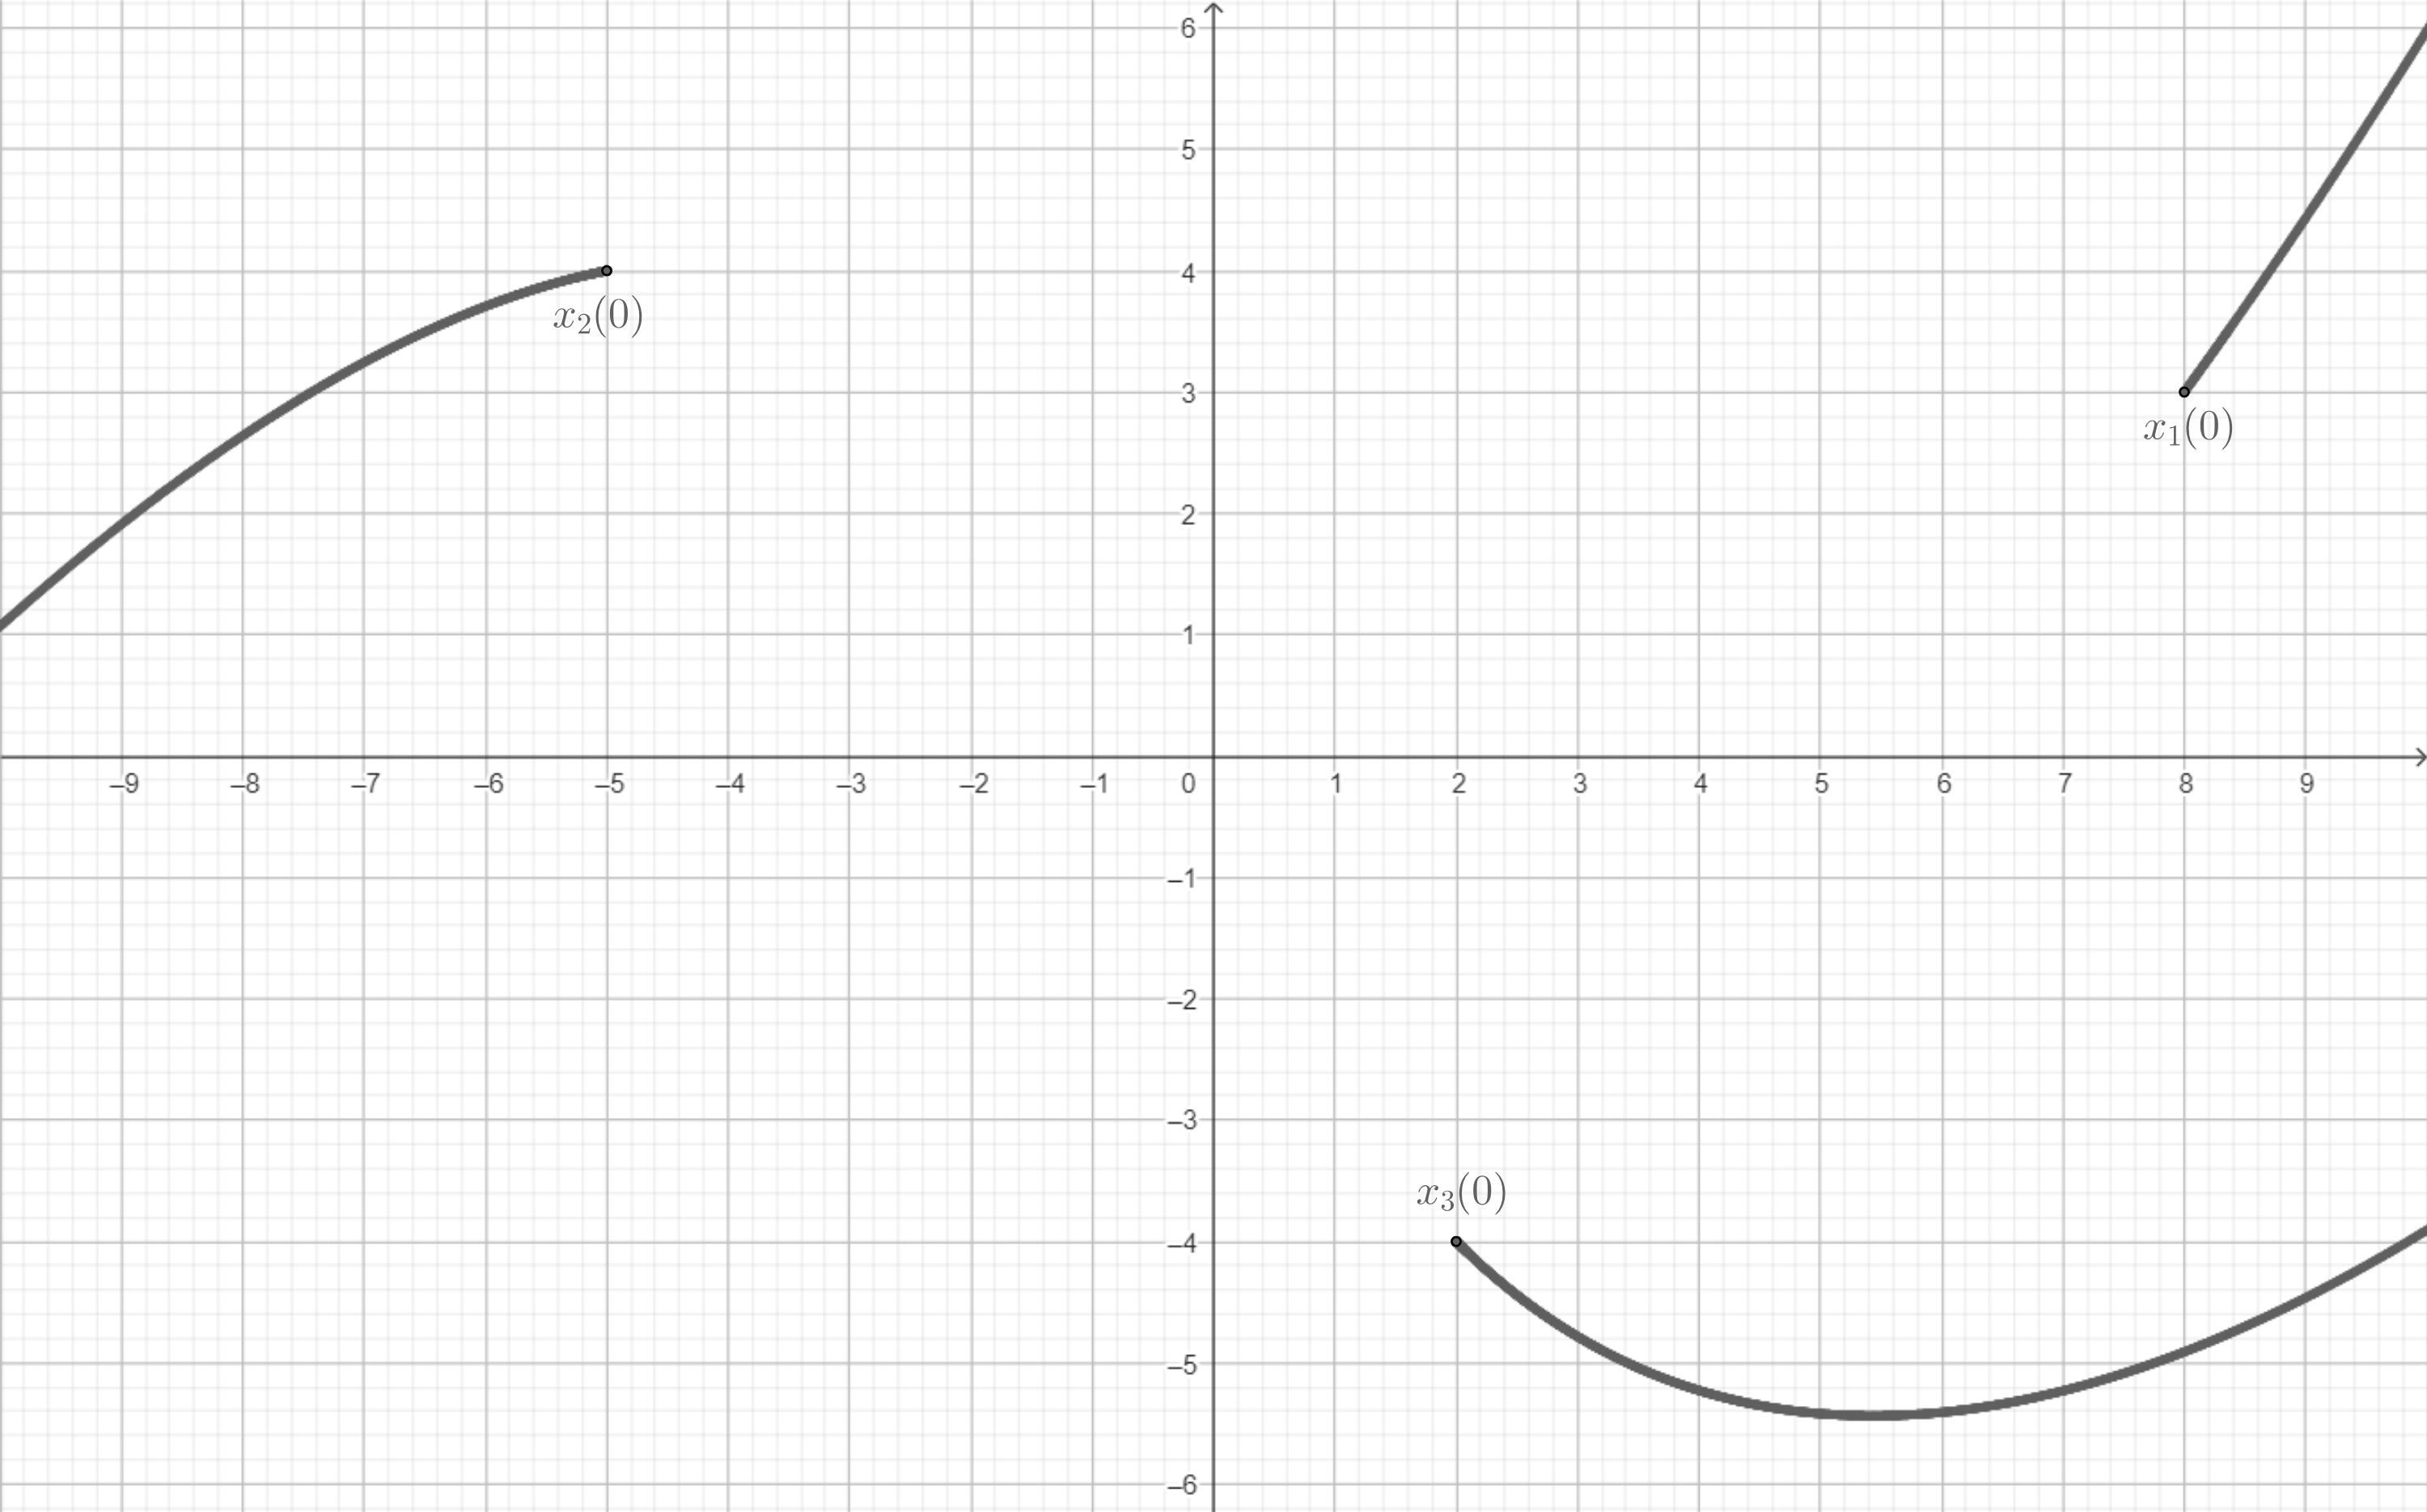
\includegraphics[width=0.45\textwidth]{2.2.png}
\end{wrapfigure}
$$\begin{bmatrix}
    x_1(t) \\ x_2(t)
\end{bmatrix} = e^{\left[\begin{smallmatrix}
    1 & 0 \\ 1 & 1
\end{smallmatrix}\right]t}\begin{bmatrix}
    a \\ b
\end{bmatrix} = \begin{bmatrix}
    e^t & 0 \\ t e^t & e^t
\end{bmatrix}\begin{bmatrix}
    a \\ b
\end{bmatrix} = \begin{bmatrix}
    ae^t \\ ate^t + be^t
\end{bmatrix}$$
Получаем для каждого из начальных условий векторы: $$\begin{bmatrix}
    ae^t \\ ate^t + be^t
\end{bmatrix} \& \begin{bmatrix}
    a = 8 \\ b = 3
\end{bmatrix} \rightarrow \begin{bmatrix}
    8e^t \\ 8te^t + 3e^t
\end{bmatrix}$$$$\begin{bmatrix}
    ae^t \\ ate^t + be^t
\end{bmatrix} \& \begin{bmatrix}
    a=-5 \\b= 4
\end{bmatrix} \rightarrow \begin{bmatrix}
    -5e^t \\ -5te^t + 4e^t
\end{bmatrix}$$
$$\begin{bmatrix}
    ae^t \\ ate^t + be^t
\end{bmatrix} \& \begin{bmatrix}
    a=2 \\ b=-4
\end{bmatrix} \rightarrow \begin{bmatrix}
    2e^t \\ 2te^t - 4e^t
\end{bmatrix}$$
Все три точки из начальных условий движутся с течением времени от центра в бесконечность --- это подтверждает, что система неустойчива.
\subsubsection*{Пункт №3}
$$\begin{bmatrix}
    x_1(t) \\ x_2(t)
\end{bmatrix} = e^{\left[\begin{smallmatrix}
    \nicefrac{4}{3} & \nicefrac{-2}{3} \\ \nicefrac{-4}{3} & \nicefrac{2}{3}
\end{smallmatrix}\right]t}\begin{bmatrix}
    a \\ b
\end{bmatrix} = \begin{bmatrix}
    \frac{2e^{2t}+1}{3} & \frac{-e^{2t}+1}{3} \\ \frac{-2e^{2t}+2}{3} & \frac{e^{2t}+2}{3}
\end{bmatrix}\begin{bmatrix}
    a \\ b
\end{bmatrix} = \begin{bmatrix}
    \frac{(2a-b)e^{2t}+a+b}{3} \\ \frac{(b-2a)e^{2t}+2(a+b)}{3}
\end{bmatrix}$$
\begin{wrapfigure}[14]{r}{0.5\textwidth}
    \centering
    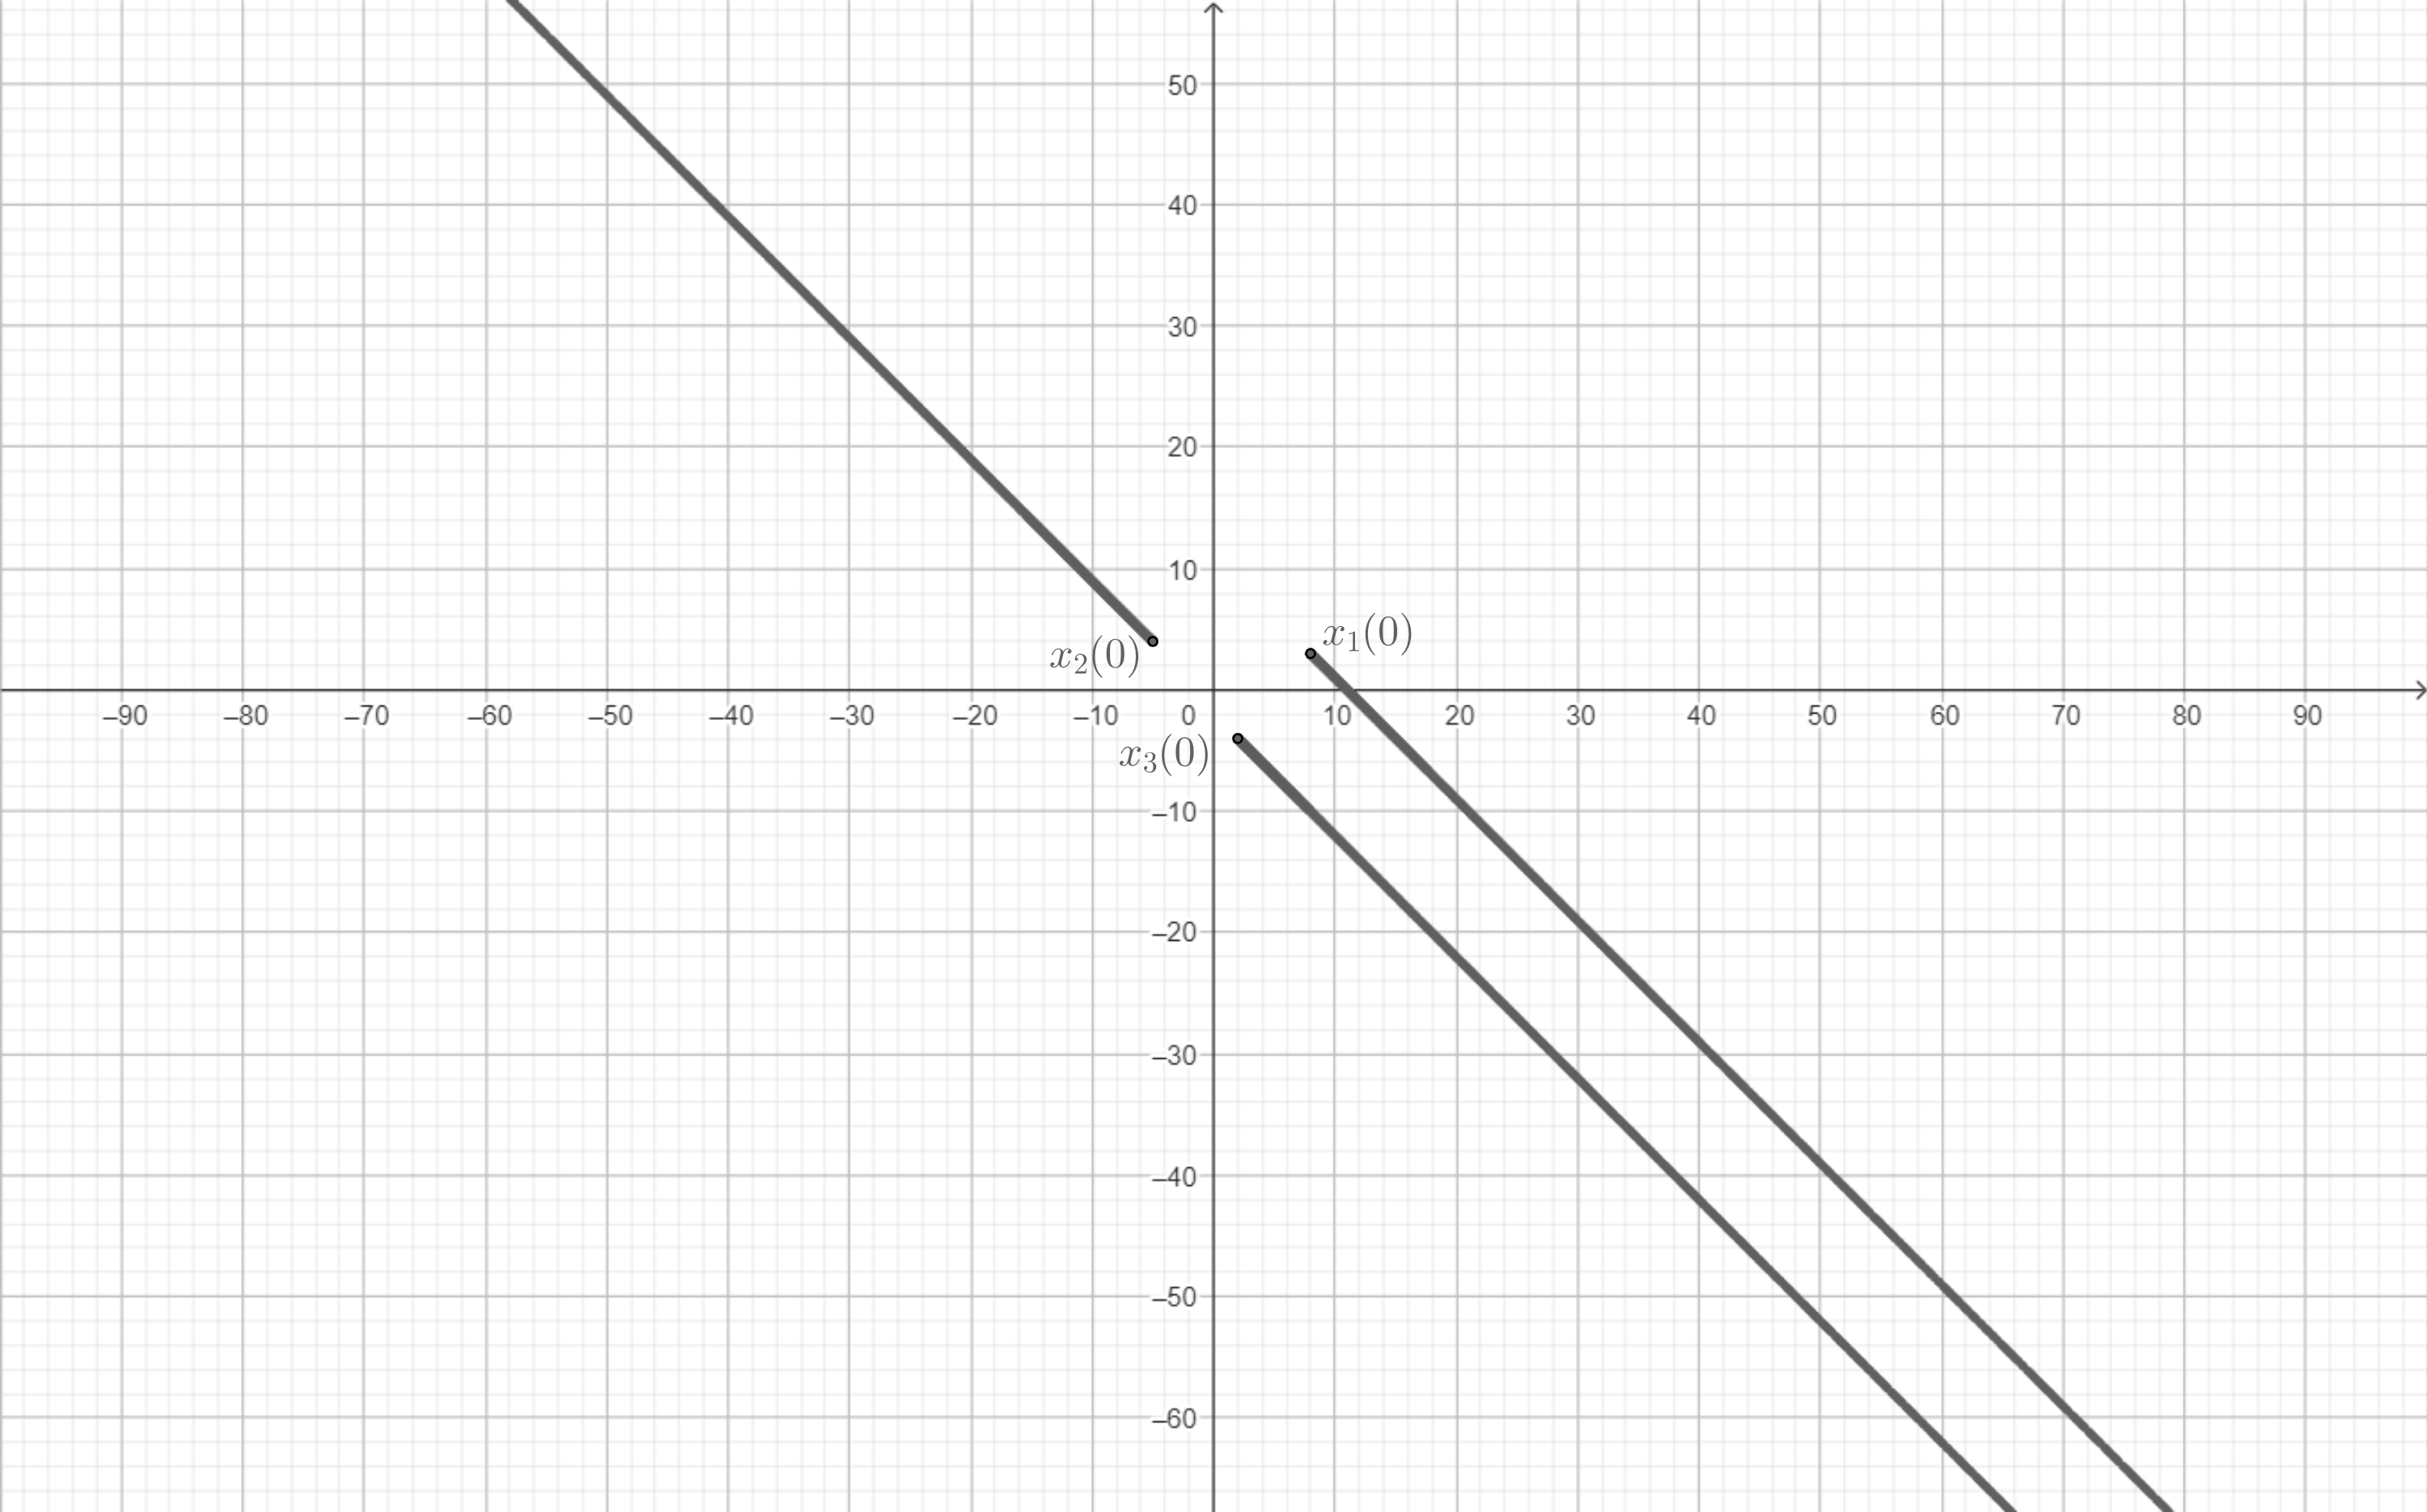
\includegraphics[width=0.5\textwidth]{2.3.png}
\end{wrapfigure}
Получаем для каждого из начальных условий векторы: $$\begin{bmatrix}
    \frac{(2a-b)e^{2t}+a+b}{3} \\ \frac{(b-2a)e^{2t}+2(a+b)}{3}
\end{bmatrix} \& \begin{bmatrix}
    a = 8 \\ b = 3
\end{bmatrix} \rightarrow \begin{bmatrix}
    \frac{13e^{2t}+11}{3} \\ \frac{-13e^{2t}+22}{3}
\end{bmatrix}$$
$$\begin{bmatrix}
    \frac{(2a-b)e^{2t}+a+b}{3} \\ \frac{(b-2a)e^{2t}+2(a+b)}{3}
\end{bmatrix} \& \begin{bmatrix}
    a=-5 \\b= 4
\end{bmatrix} \rightarrow \begin{bmatrix}
    \frac{-14e^{2t}-1}{3} \\ \frac{14e^{2t}-2}{3}
\end{bmatrix}$$
$$\begin{bmatrix}
    \frac{(2a-b)e^{2t}+a+b}{3} \\ \frac{(b-2a)e^{2t}+2(a+b)}{3}
\end{bmatrix} \& \begin{bmatrix}
    a=2 \\ b=-4
\end{bmatrix} \rightarrow \begin{bmatrix}
    \frac{8e^{2t}-2}{3} \\ \frac{-8e^{2t}-4}{3}
\end{bmatrix}$$
Заметим, что точка с начальным условием $x_1(0)$ при движении в бесконечности немного склоняется влево --- это говорит о том, что система неустойчива, но при это по второму собственному вектору системы. Если бы одно из начальных условий лежало бы на первом собственном векторе, то динамическая система сжала бы его в ноль.
\subsubsection*{Пункт №4}
$$\begin{bmatrix}
    x_1(t) \\ x_2(t)
\end{bmatrix} = e^{\left[\begin{smallmatrix}
    0 & 5 \\ -2 & -2
\end{smallmatrix}\right]t}\begin{bmatrix}
    a \\ b
\end{bmatrix} = \begin{bmatrix}
    \frac{3\cos{3t}-i\sin{3t}}{3e^t} & \frac{4i\sin{3t}}{3e^t} \\
    \frac{2i\sin{3t}}{3e^t} & \frac{3\cos{3t}+i\sin{3t}}{3e^t}
\end{bmatrix}\begin{bmatrix}
    a \\ b
\end{bmatrix} = \begin{bmatrix}
    \frac{3a\cos{3t}-(4b-a)i\sin{3t}}{3e^t} \\ \frac{3b\cos{3t}+(2a+b)i\sin{3t}}{3e^t}
\end{bmatrix}$$
\begin{wrapfigure}[12]{r}{0.35\textwidth}
    \centering
    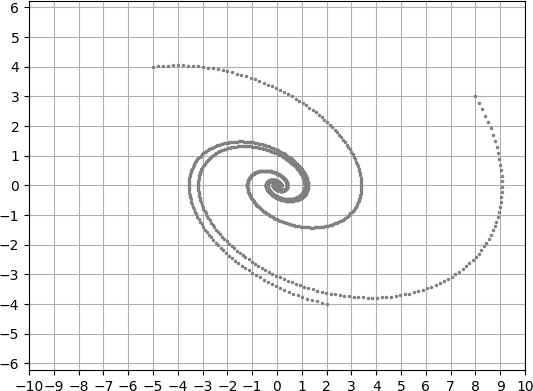
\includegraphics[width=0.35\textwidth]{2.4.png}
\end{wrapfigure}
Получаем для каждого из начальных условий векторы: $$\begin{bmatrix}
    \frac{3a\cos{3t}-(4b-a)i\sin{3t}}{3e^t} \\ \frac{3b\cos{3t}+(2a+b)i\sin{3t}}{3e^t}
\end{bmatrix} \& \begin{bmatrix}
    a = 8 \\ b = 3
\end{bmatrix} \rightarrow \begin{bmatrix}
    \frac{24\cos{3t}-29i\sin{3t}}{3e^t} \\ \frac{9\cos{3t}+19i\sin{3t}}{3e^t}
\end{bmatrix}$$
$$\begin{bmatrix}
    \frac{3a\cos{3t}-(4b-a)i\sin{3t}}{3e^t} \\ \frac{3b\cos{3t}+(2a+b)i\sin{3t}}{3e^t}
\end{bmatrix} \& \begin{bmatrix}
    a=-5 \\b= 4
\end{bmatrix} \rightarrow \begin{bmatrix}
    \frac{-5\cos{3t}-7i\sin{3t}}{e^t} \\ \frac{4\cos{3t}-2i\sin{3t}}{e^t}
\end{bmatrix}$$
$$\begin{bmatrix}
    \frac{3a\cos{3t}-(4b-a)i\sin{3t}}{3e^t} \\ \frac{3b\cos{3t}+(2a+b)i\sin{3t}}{3e^t}
\end{bmatrix} \& \begin{bmatrix}
    a=2 \\ b=-4
\end{bmatrix} \rightarrow \begin{bmatrix}
    \frac{2\cos{3t}+6i\sin{3t}}{e^t} \\ \frac{-4\cos{3t}}{e^t}
\end{bmatrix}$$
Наблюдается стремление точек динамической системы к нулю, что подтверждает её асимптотическую устойчивость. \\[0.5em]
\NB: для расчёта фазовых траекторий для $x_1(t)$ и $x_2(t)$, содержащих в себе комплексные числа, \verb|GeoGebra| не подходит, поэтому здесь и в следующем пункте используется визуализация модуля \verb|Matplotlib| из \textbf{Python}.
\pagebreak
\subsubsection*{Пункт №5}
$$\begin{bmatrix}
    x_1(t) \\ x_2(t)
\end{bmatrix} = e^{\left[\begin{smallmatrix}
    2 & 5 \\ -2 & 0
\end{smallmatrix}\right]t}\begin{bmatrix}
    a \\ b
\end{bmatrix} = \begin{bmatrix}
    \frac{e^t(3\cos{3t}+i\sin{3t})}{3} & \frac{-4ie^t\sin{3t}}{3} \\
    \frac{-2ie^t\sin{3t}}{3} & \frac{e^t(3\cos{3t}-i\sin{3t})}{3}
\end{bmatrix}\begin{bmatrix}
    a \\ b
\end{bmatrix} = \begin{bmatrix}
    \frac{e^t(3a\cos{3t}+(a-4b)i\sin{3t})}{3} \\
    \frac{e^t(3b\cos{3t}-(2a+b)i\sin{3t})}{3}
\end{bmatrix}$$
\begin{wrapfigure}[9]{r}{0.34\textwidth}
    \centering
    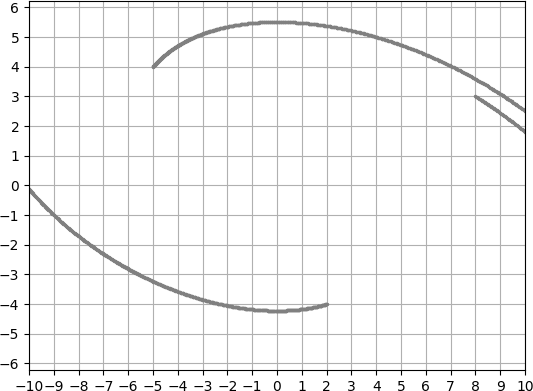
\includegraphics[width=0.34\textwidth]{2.6.png}
\end{wrapfigure}
Получаем для каждого из начальных условий векторы: $$\begin{bmatrix}
    \frac{e^t(3a\cos{3t}+(a-4b)i\sin{3t})}{3} \\
    \frac{e^t(3b\cos{3t}-(2a+b)i\sin{3t})}{3}
\end{bmatrix} \& \begin{bmatrix}
    a = 8 \\ b = 3
\end{bmatrix} \rightarrow \begin{bmatrix}
    \frac{e^t(24\cos{3t}-4i\sin{3t})}{3} \\
    \frac{e^t(9\cos{3t}-19i\sin{3t})}{3}
\end{bmatrix}$$
$$\begin{bmatrix}
    \frac{e^t(3a\cos{3t}+(a-4b)i\sin{3t})}{3} \\
    \frac{e^t(3b\cos{3t}-(2a+b)i\sin{3t})}{3}
\end{bmatrix} \& \begin{bmatrix}
    a=-5 \\b= 4
\end{bmatrix} \rightarrow \begin{bmatrix}
    e^t(-5\cos{3t}-7i\sin{3t}) \\
    e^t(4\cos{3t}+2i\sin{3t})
\end{bmatrix}$$
$$\begin{bmatrix}
    \frac{e^t(3a\cos{3t}+(a-4b)i\sin{3t})}{3} \\
    \frac{e^t(3b\cos{3t}-(2a+b)i\sin{3t})}{3}
\end{bmatrix} \& \begin{bmatrix}
    a=2 \\ b=-4
\end{bmatrix} \rightarrow \begin{bmatrix}
    e^t(2\cos{3t}+6i\sin{3t}) \\
    -4e^t\cos{3t}
\end{bmatrix}$$
Все точки убежали с графика, что говорит о том, что система неустойчива.
\subsubsection*{Пункт №6}
$$\begin{bmatrix}
    x_1(t) \\ x_2(t)
\end{bmatrix} = e^{\left[\begin{smallmatrix}
    1 & 5 \\ -2 & -1
\end{smallmatrix}\right]t}\begin{bmatrix}
    a \\ b
\end{bmatrix} = \begin{bmatrix}
    \cos{3t}-\sin{3t} & -\sin{3t} \\ 0 & \cos{3t}+\sin{3t}
\end{bmatrix}\begin{bmatrix}
    a \\ b
\end{bmatrix} = \begin{bmatrix}
    a\cos{3t}-(a+b)\sin{3t} \\ b\cos{3t}-b\sin{3t}
\end{bmatrix}$$
\begin{wrapfigure}[13]{r}{0.354\textwidth}
    \centering
    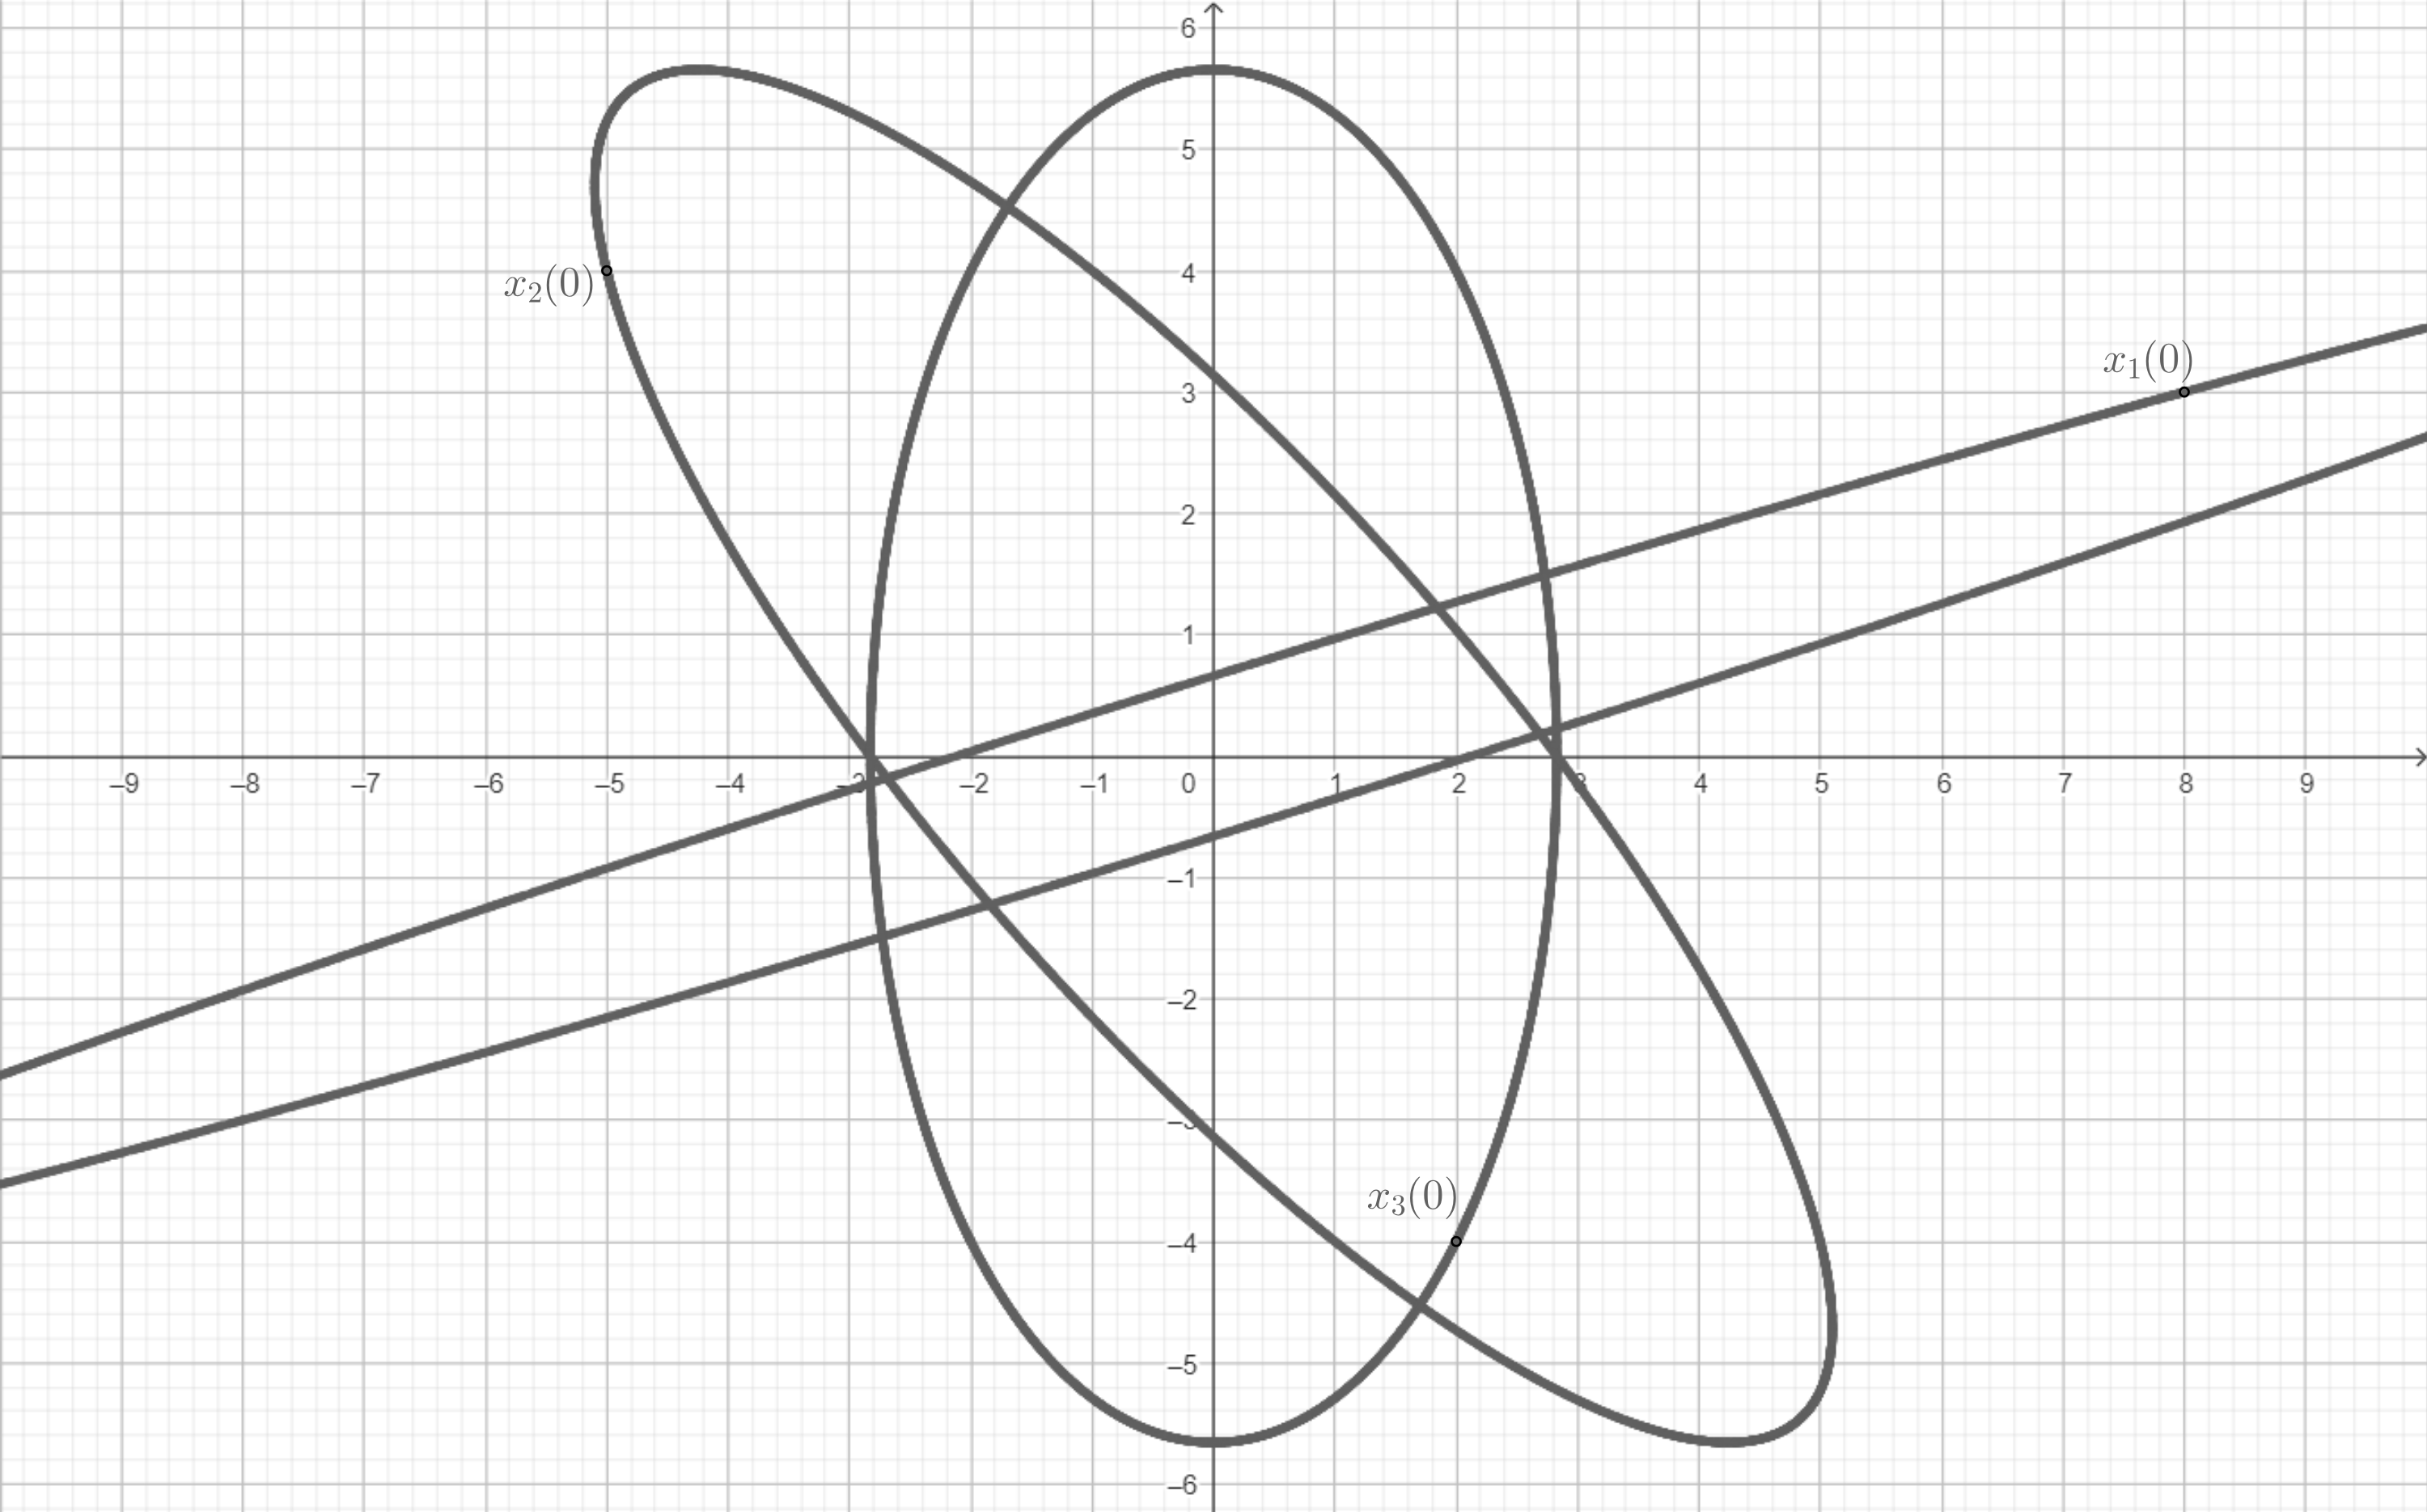
\includegraphics[width=0.35\textwidth]{2.5.png}
\end{wrapfigure}
Получаем для каждого из начальных условий векторы: $$\begin{bmatrix}
    a\cos{3t}-(a+b)\sin{3t} \\ b\cos{3t}-b\sin{3t}
\end{bmatrix} \& \begin{bmatrix}
    a = 8 \\ b = 3
\end{bmatrix} \rightarrow \begin{bmatrix}
    8\cos{3t}-11\sin{3t} \\ 3\cos{3t}-3\sin{3t}
\end{bmatrix}$$
$$\begin{bmatrix}
    a\cos{3t}-(a+b)\sin{3t} \\ b\cos{3t}-b\sin{3t}
\end{bmatrix} \& \begin{bmatrix}
    a=-5 \\b= 4
\end{bmatrix} \rightarrow \begin{bmatrix}
    \sin{3t}-5\cos{3t} \\ 4\cos{3t}-4\sin{3t}
\end{bmatrix}$$
$$\begin{bmatrix}
    a\cos{3t}-(a+b)\sin{3t} \\ b\cos{3t}-b\sin{3t}
\end{bmatrix} \& \begin{bmatrix}
    a=2 \\ b=-4
\end{bmatrix} \rightarrow \begin{bmatrix}
    2\cos{3t}+2\sin{3t} \\ 4\sin{3t}-4\cos{3t}
\end{bmatrix}$$\,\\[0em]
Прекрасные эллипсы на наших глазах говорят о замкнутости траектории движения точек в динамической системе --- система устойчива, но не асимптотически.
\subsection*{\centering Задание №3. Дискретку автоматом закрыл}
Придумаем две константы $c = 0.5$ и $d = 3$ для выполнения этого задания.
\subsubsection*{Пункт №1}
Перед нами встаёт выбор, какую матрицу выбрать: $\left[\begin{smallmatrix}
    -1 & 0 \\ 0 & -1
\end{smallmatrix}\right]$ или $\left[\begin{smallmatrix}
    -1 & 1 \\ 0 & -1
\end{smallmatrix}\right]$. Первую мы не можем выбрать, т.к. она диагональная и при перемножении с базисом собственных векторов даст нам саму себя же, а у нас важное условие --- придуманные матрицы не должны быть диагональными, поэтому выбираем вторую. Базис собственных векторов выберём наугад:
$$A = PJP^{-1} = \begin{bmatrix}
    1 & 2 \\ 3 & 4
\end{bmatrix}\begin{bmatrix}
    -1 & 1 \\ 0 & -1
\end{bmatrix}\begin{bmatrix}
    1 & 2 \\ 3 & 4
\end{bmatrix}^{-1} = \begin{bmatrix}
    \nicefrac{1}{2} & \nicefrac{-1}{2} \\
    \nicefrac{9}{2} & \nicefrac{-5}{2}
\end{bmatrix}$$
\subsubsection*{Пункт №2}
Если перед нами комплексные числа, то выбрать такие собственные вектора, чтобы матрица оказалась в поле вещественных чисел, очень просто --- необходимо выбрать два вектора, которые будут отличаться лишь комплексно сопряжёнными числами. Ниже пример:
$$A = PDP^{-1} = \begin{bmatrix}
    1+i & 1-i \\ 1 & 1
\end{bmatrix}\begin{bmatrix}
    \nicefrac{-1}{\sqrt{2}}+\nicefrac{1}{\sqrt{2}}i & 0 \\ 0 & \nicefrac{-1}{\sqrt{2}}-\nicefrac{1}{\sqrt{2}}i
\end{bmatrix}\begin{bmatrix}
    1+i & 1-i \\ 1 & 1
\end{bmatrix}^{-1} = \begin{bmatrix}
    0 & -\sqrt{2} \\ \nicefrac{\sqrt{2}}{2} & -\sqrt{2}
\end{bmatrix}$$
\subsubsection*{Пункт №3}
Проворачиваем похожий трюк с собственными векторами, но выберем другие для разнообразия:
$$A = PDP^{-1} = \begin{bmatrix}
    i & -i \\ 1 & 1
\end{bmatrix}\begin{bmatrix}
    i & 0 \\ 0 & -i
\end{bmatrix}\begin{bmatrix}
    i & -i \\ 1 & 1
\end{bmatrix}^{-1} = \begin{bmatrix}
    0 & -1 \\ 1 & 0
\end{bmatrix}$$
Отмечу, что матрица не диагональная, т.к. по определению диагональная матрица --- матрица, у которого ненулевые элементы расположены \underline{только} на главной диагонали.
\subsubsection*{Пункт №4}
Не будем сильно крутиться-вертеться и просто подставим те же самые собственные вектора, что и в пункте №2:
$$A = PDP^{-1} = \begin{bmatrix}
    1+i & 1-i \\ 1 & 1
\end{bmatrix}\begin{bmatrix}
    \nicefrac{1}{\sqrt{2}}+\nicefrac{1}{\sqrt{2}}i & 0 \\ 0 & \nicefrac{1}{\sqrt{2}}-\nicefrac{1}{\sqrt{2}}i
\end{bmatrix}\begin{bmatrix}
    1+i & 1-i \\ 1 & 1
\end{bmatrix}^{-1} = \begin{bmatrix}
    \sqrt{2} & -\sqrt{2} \\ \nicefrac{\sqrt{2}}{2} & 0
\end{bmatrix}$$
\subsubsection*{Пункт №5}
Здесь имеем ситуацию, подобную той, что была в пункте №1 --- нам необходимо выбрать не диагональную матрицу собственных чисел, а жорданову форму:
$$A = PJP^{-1} = \begin{bmatrix}
    1 & 2 \\ 3 & 4
\end{bmatrix}\begin{bmatrix}
    1 & 1 \\ 0 & 1
\end{bmatrix}\begin{bmatrix}
    1 & 2 \\ 3 & 4
\end{bmatrix}^{-1} = \begin{bmatrix}
    \nicefrac{5}{2} & \nicefrac{-1}{2} \\
    \nicefrac{9}{2} & \nicefrac{-1}{2}
\end{bmatrix}$$
\subsubsection*{Пункт №6}
Теперь перед нами собственные числа $\lambda_{1,2} = -0.5$, но алгоритм получения матрицы $A$ тот же:
$$A = PJP^{-1} = \begin{bmatrix}
    1 & 2 \\ 3 & 4
\end{bmatrix}\begin{bmatrix}
    -0.5 & 1 \\ 0 & -0.5
\end{bmatrix}\begin{bmatrix}
    1 & 2 \\ 3 & 4
\end{bmatrix}^{-1} = \begin{bmatrix}
    1 & \nicefrac{-1}{2} \\
    \nicefrac{9}{2} & -2
\end{bmatrix}$$
\subsubsection*{Пункт №7}
Здесь имеем собственные числа $\lambda_{1,2}= \pm0.5i$:
$$A = PDP^{-1} = \begin{bmatrix}
    i & -i \\ 1 & 1
\end{bmatrix}\begin{bmatrix}
    0.5i & 0 \\ 0 & -0.5i
\end{bmatrix}\begin{bmatrix}
    i & -i \\ 1 & 1
\end{bmatrix}^{-1} = \begin{bmatrix}
    0 & \nicefrac{-1}{2} \\ \nicefrac{1}{2} & 0
\end{bmatrix}$$
\subsubsection*{Пункт №8}
В диагональной матрице работаем с собственными числами $\lambda_{1,2}= 0.5$:
$$A = PJP^{-1} = \begin{bmatrix}
    1 & 2 \\ 3 & 4
\end{bmatrix}\begin{bmatrix}
    0.5 & 1 \\ 0 & 0.5
\end{bmatrix}\begin{bmatrix}
    1 & 2 \\ 3 & 4
\end{bmatrix}^{-1} = \begin{bmatrix}
    2 & \nicefrac{-1}{2} \\
    \nicefrac{9}{2} & -1
\end{bmatrix}$$
\subsubsection*{Пункт №9}
Теперь перед нами собственные числа $\lambda_{1,2} = -3$, но алгоритм получения матрицы $A$ тот же:
$$A = PJP^{-1} = \begin{bmatrix}
    1 & 2 \\ 3 & 4
\end{bmatrix}\begin{bmatrix}
    -3 & 1 \\ 0 & -3
\end{bmatrix}\begin{bmatrix}
    1 & 2 \\ 3 & 4
\end{bmatrix}^{-1} = \begin{bmatrix}
    \nicefrac{-3}{2} & \nicefrac{-1}{2} \\
    \nicefrac{9}{2} & \nicefrac{-9}{2}
\end{bmatrix}$$
\subsubsection*{Пункт №10}
Здесь имеем собственные числа $\lambda_{1,2}= \pm3i$:
$$A = PDP^{-1} = \begin{bmatrix}
    i & -i \\ 1 & 1
\end{bmatrix}\begin{bmatrix}
    3i & 0 \\ 0 & -3i
\end{bmatrix}\begin{bmatrix}
    i & -i \\ 1 & 1
\end{bmatrix}^{-1} = \begin{bmatrix}
    0 & -3 \\ 3 & 0
\end{bmatrix}$$
\subsubsection*{Пункт №11}
В диагональной матрице работаем с собственными числами $\lambda_{1,2}= 3$:
$$A = PJP^{-1} = \begin{bmatrix}
    1 & 2 \\ 3 & 4
\end{bmatrix}\begin{bmatrix}
    3 & 1 \\ 0 & 3
\end{bmatrix}\begin{bmatrix}
    1 & 2 \\ 3 & 4
\end{bmatrix}^{-1} = \begin{bmatrix}
    \nicefrac{9}{2} & \nicefrac{-1}{2} \\
    \nicefrac{9}{2} & \nicefrac{3}{2}
\end{bmatrix}$$
\subsubsection*{Пункт №12}
Нас пытаются поймать в ловушку, похожую на пункты №1,5,6,8,9,11, но мы не попадёмся на неё, потому что это уже 7 раз: если мы будем использовать диагональную матрицу $\left[\begin{smallmatrix}
    0 & 0 \\ 0 & 0
\end{smallmatrix}\right]$, то у нас обнулится всё на свете и нам не выжить, поэтому нужно использовать жорданову форму, возникающую при недостатке собственных векторов матрицы $\left[\begin{smallmatrix}
    0 & 1 \\ 0 & 0
\end{smallmatrix}\right]$ --- здесь есть хоть какая-то единичка :)
$$A = PJP^{-1} = \begin{bmatrix}
    1 & 2 \\ 3 & 4
\end{bmatrix}\begin{bmatrix}
    0 & 1 \\ 0 & 0
\end{bmatrix}\begin{bmatrix}
    1 & 2 \\ 3 & 4
\end{bmatrix}^{-1} = \begin{bmatrix}
    \nicefrac{3}{2} & \nicefrac{-1}{2} \\
    \nicefrac{9}{2} & \nicefrac{-3}{2}
\end{bmatrix}$$\pagebreak

\noindent Теперь пришло время расположить все собственные числа на комплексной плокости.
\begin{figure}[h]
    \centering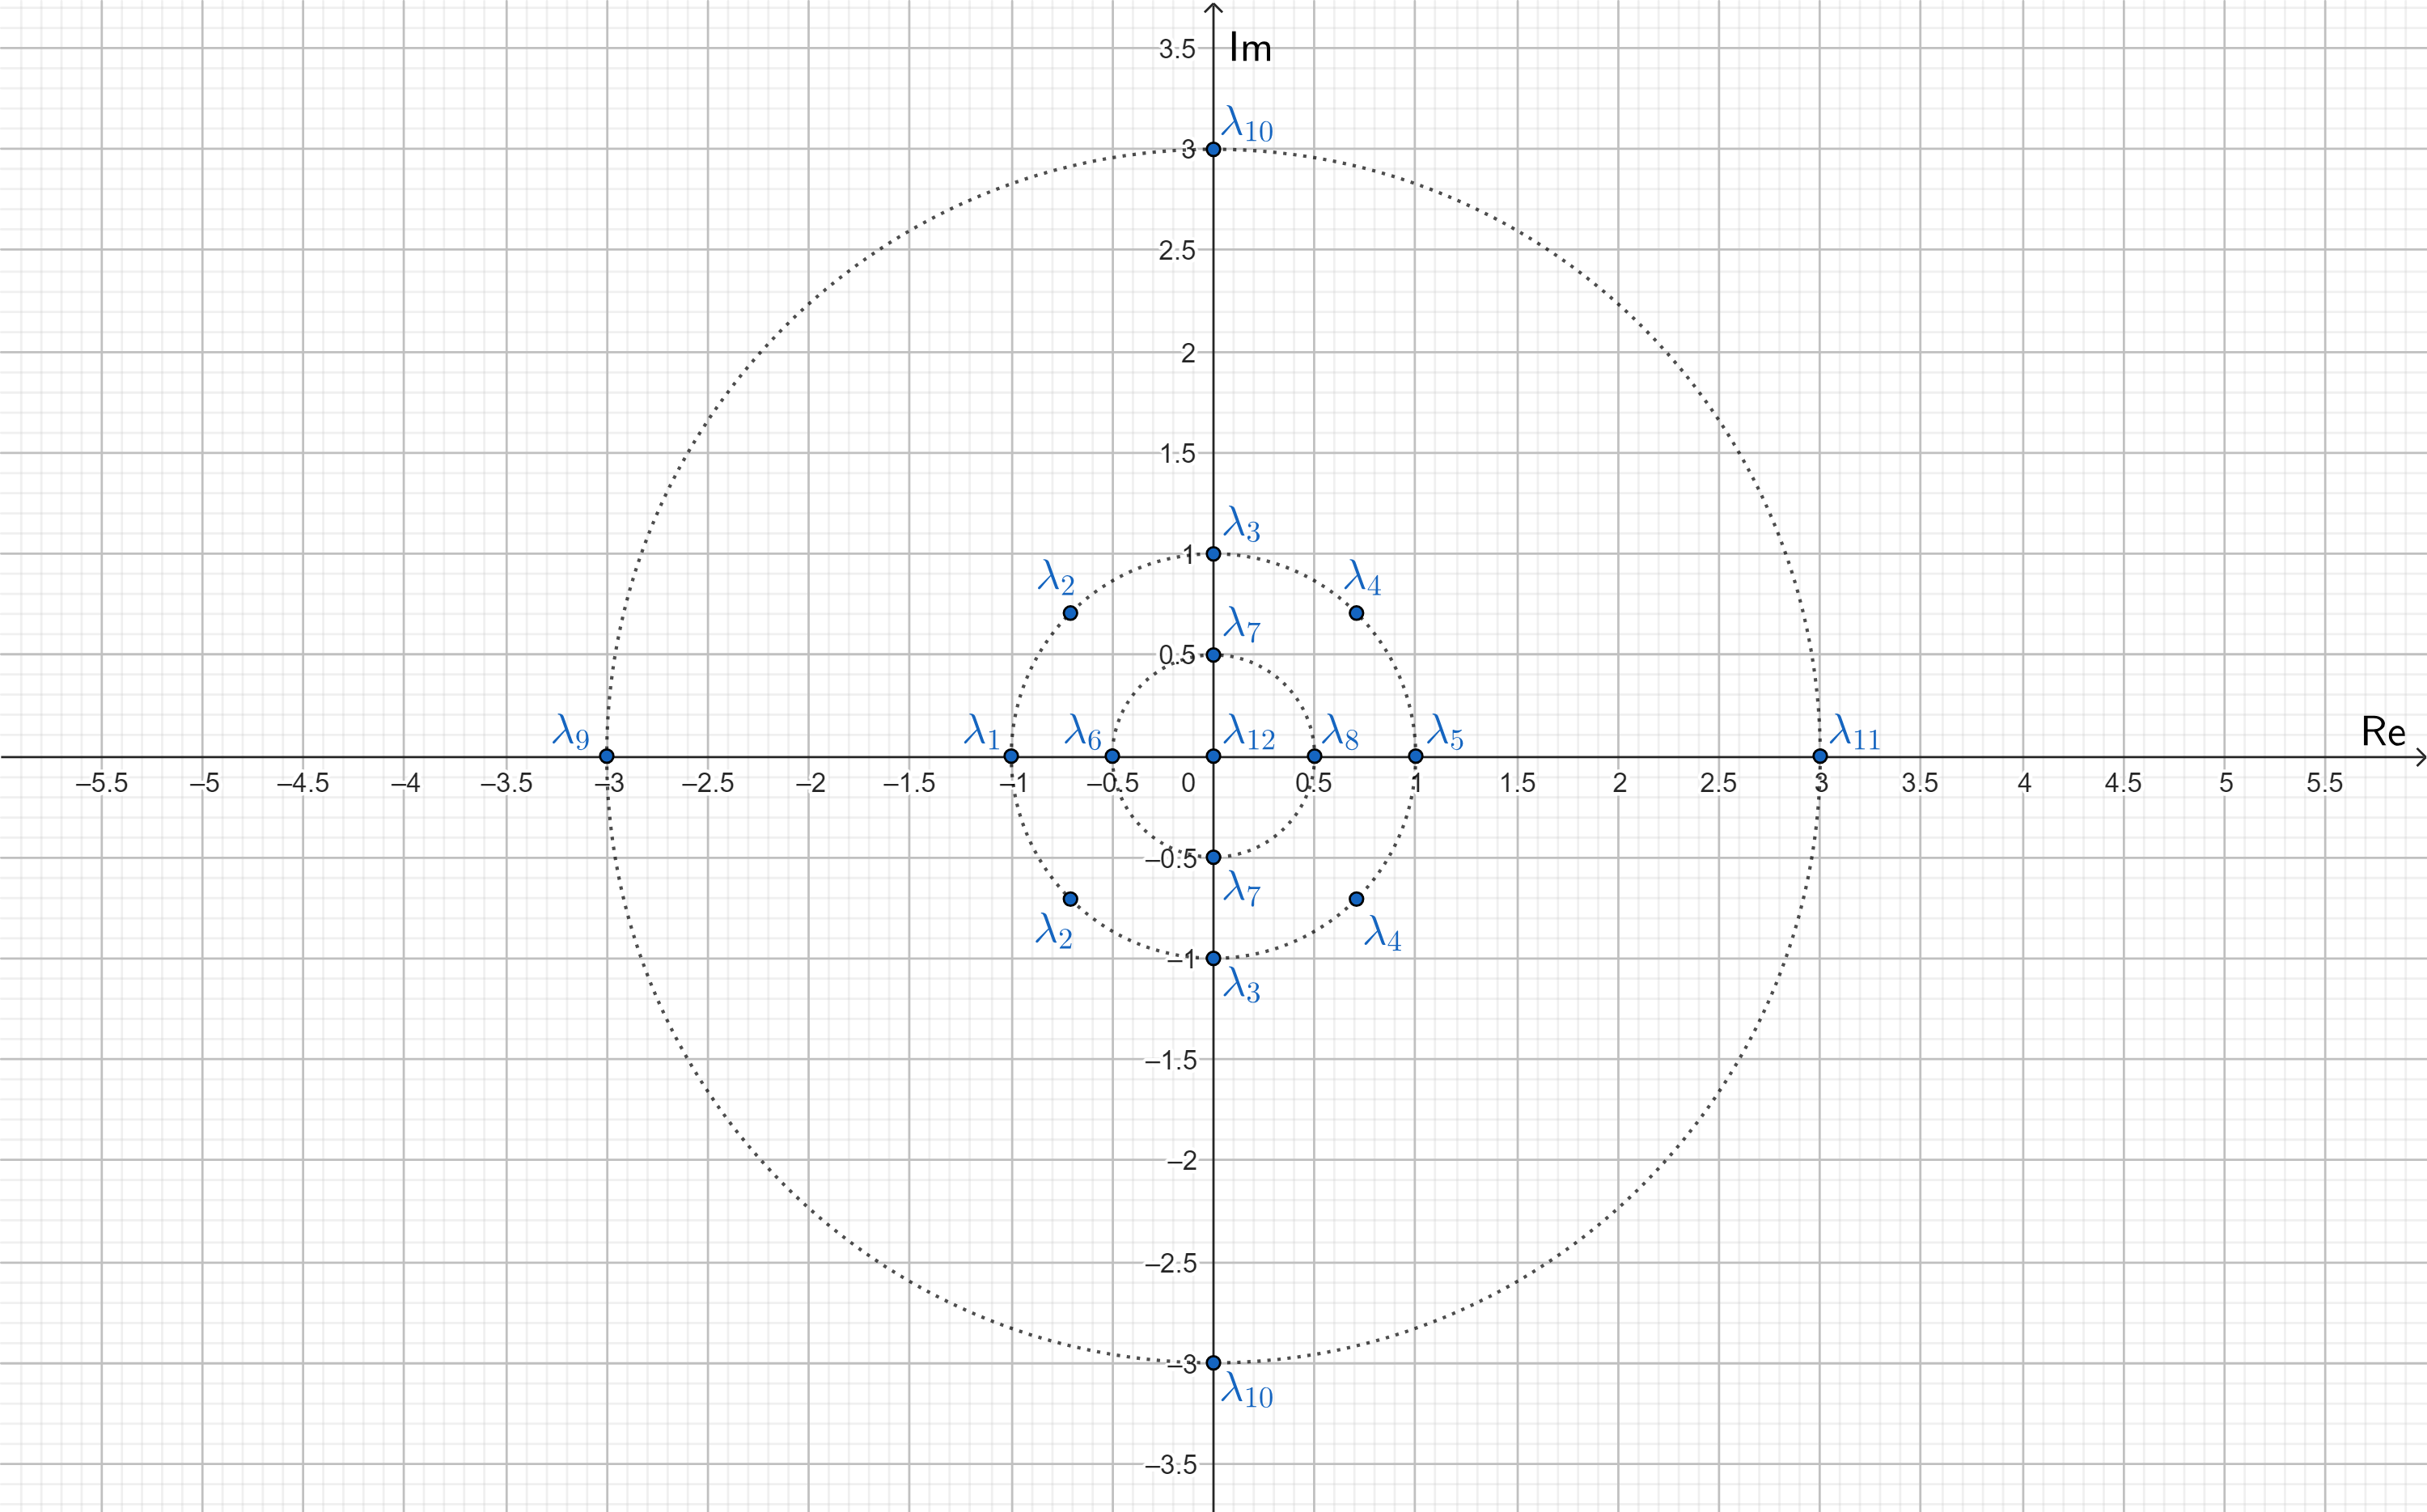
\includegraphics[width=0.5\textwidth]{3.png}
\end{figure} \\
Выясняется, что перед нами три группы собственных чисел, образующих три окружности разных радиусов.\\[2em]
\subsection*{\centering Задание №4. Таким моделям гигачад позавидует\ldots}
Зададим начальное условие $x(0) = \left[\begin{smallmatrix}
    4 \\ 2
\end{smallmatrix}\right]$ и будем проводить манипуляции, подобные тем, что были для непрерывных динамических систем.
\subsubsection*{Пункт №1}
$$\begin{bmatrix}
    x_1(k) \\ x_2(k)
\end{bmatrix} = \begin{bmatrix}
    \nicefrac{1}{2} & \nicefrac{-1}{2} \\ \nicefrac{9}{2} & \nicefrac{-5}{2}
\end{bmatrix}^k\begin{bmatrix}
    4 \\ 2
\end{bmatrix} = \begin{bmatrix}
    \frac{2\cdot(-1)^k-3\cdot(-1)^kk}{2} & \frac{(-1)^kk}{2} \\
    \frac{-9\cdot(-1)^kk}{2} & \frac{2\cdot(-1)^k+3\cdot(-1)^kk}{2}
\end{bmatrix}\begin{bmatrix}
    4 \\ 2
\end{bmatrix} = \begin{bmatrix}
    4\cdot(-1)^k-5\cdot(-1)^kk \\ 2\cdot(-1)^k-15\cdot(-1)^kk
\end{bmatrix}$$
\begin{figure}[h]
    \centering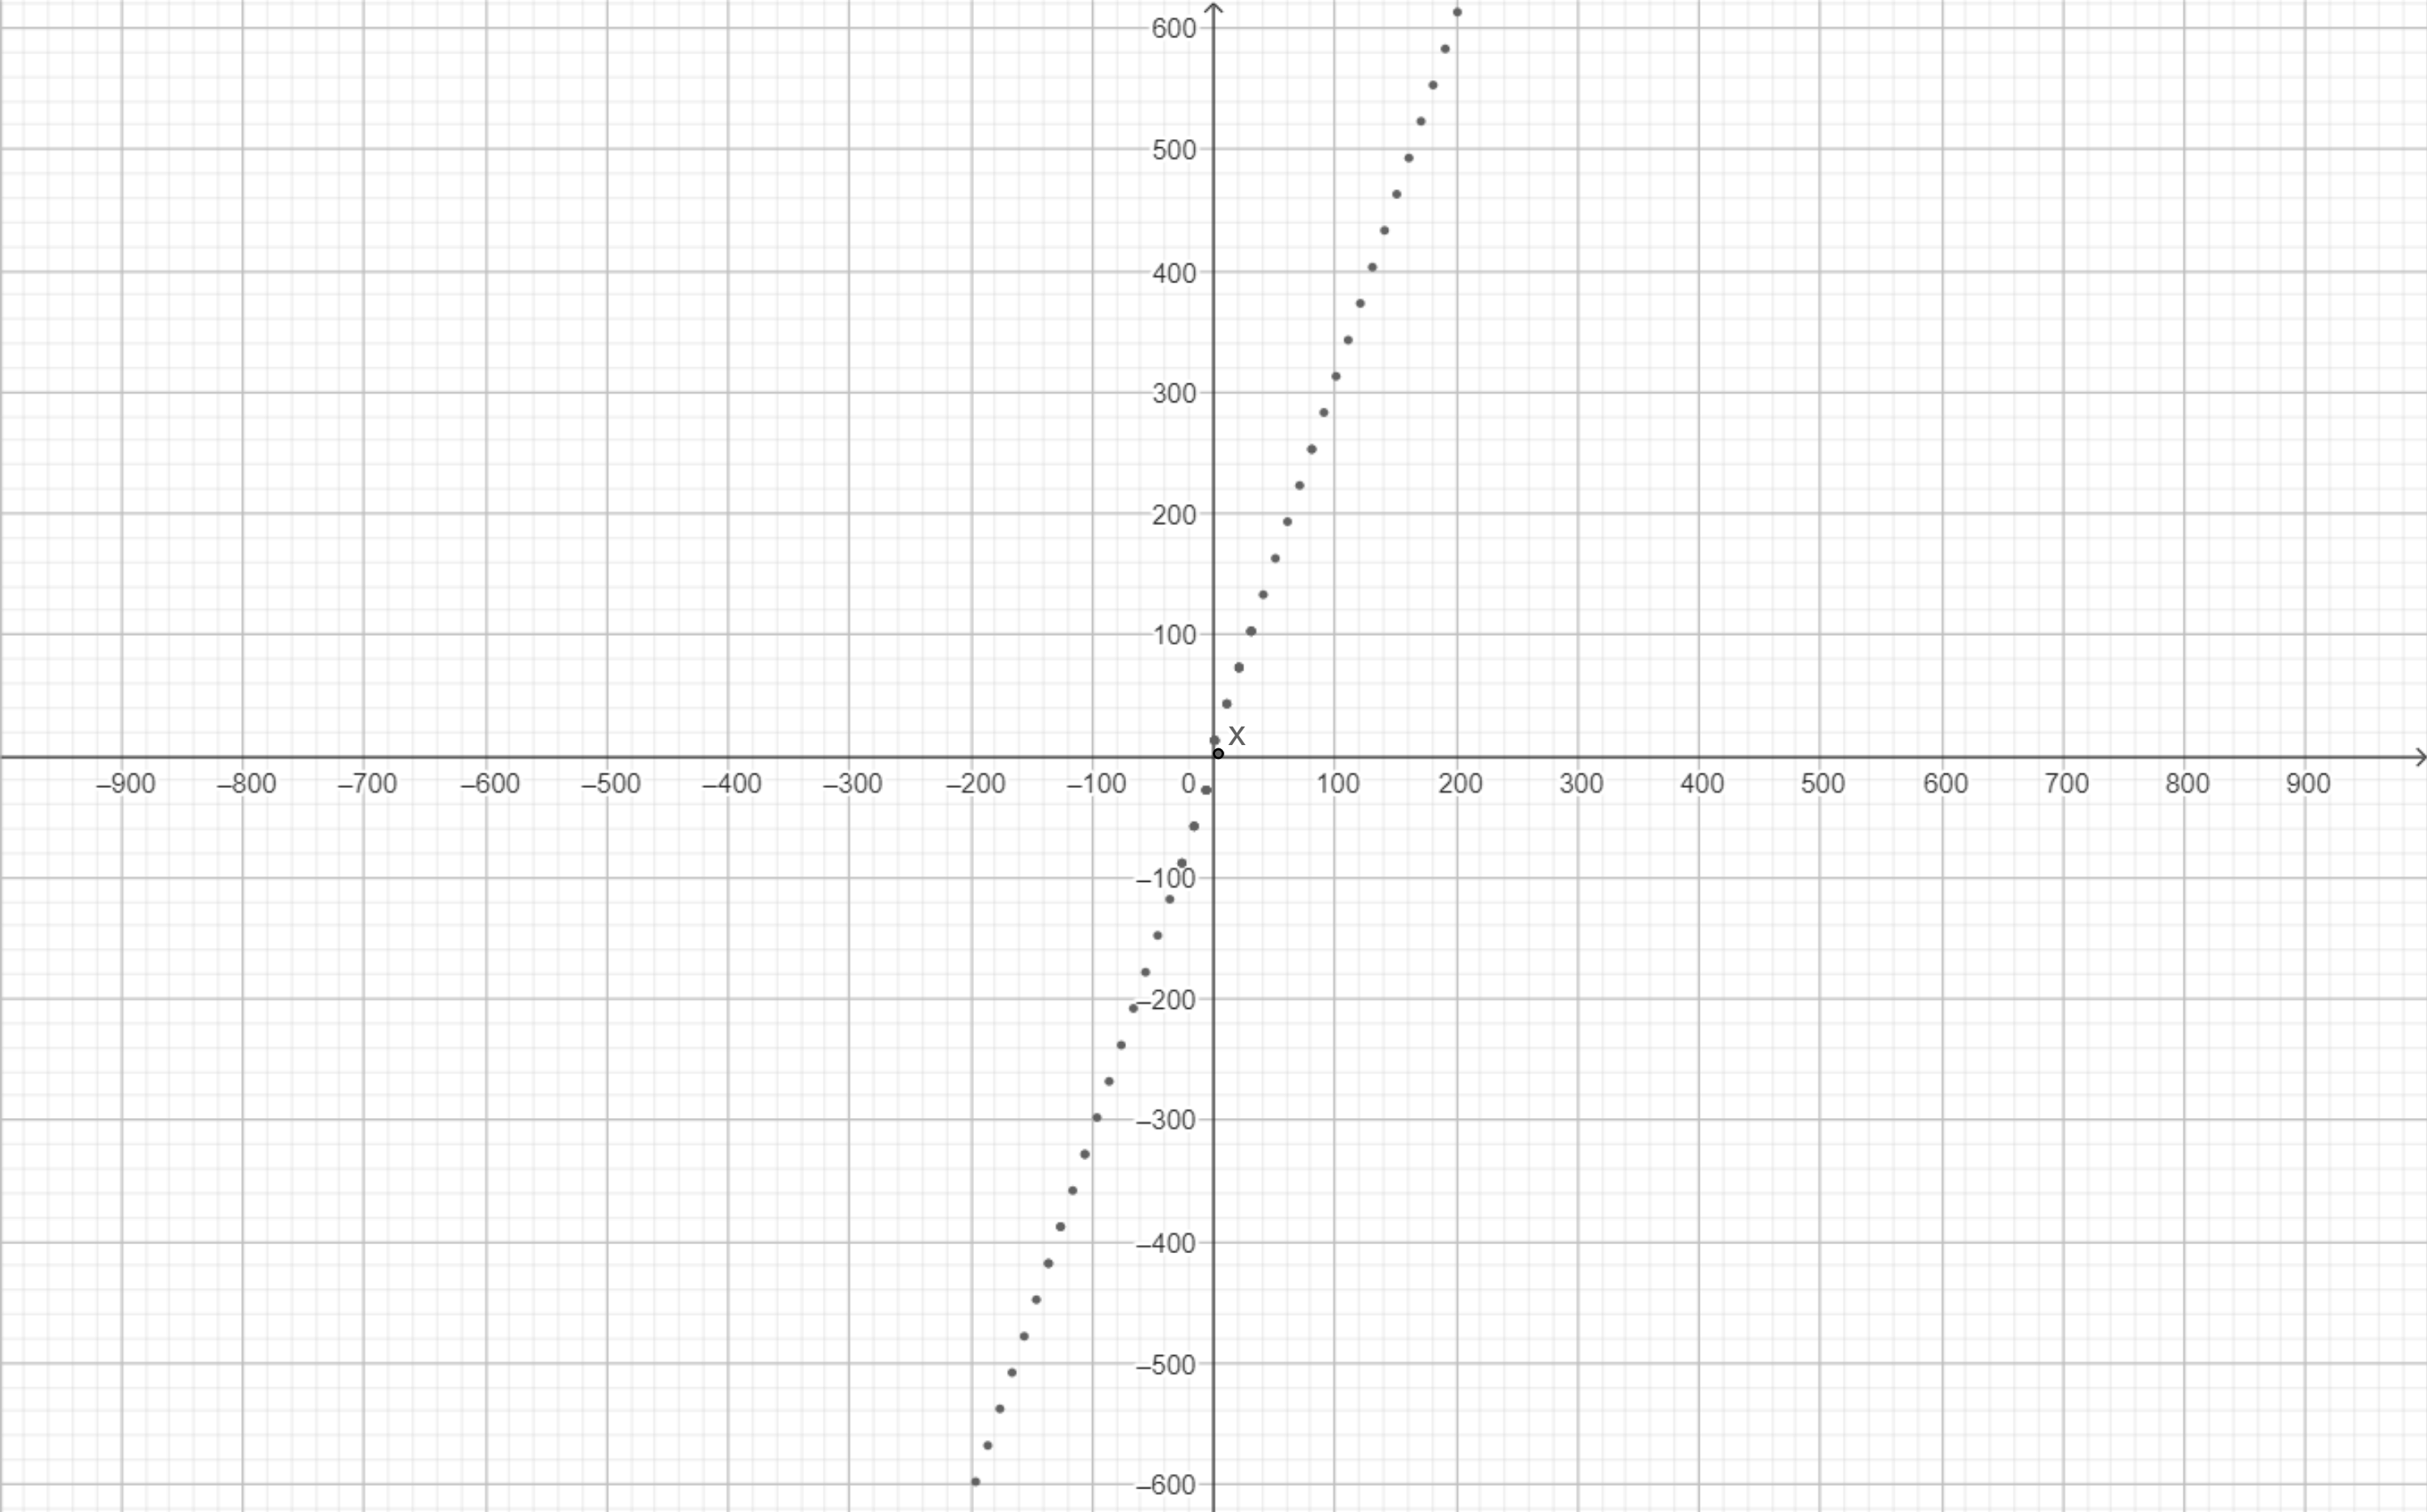
\includegraphics[width=0.5\textwidth]{4.1.png}
\end{figure} \pagebreak
\subsubsection*{Пункт №2}
$$\begin{bmatrix}
    x_1(k) \\ x_2(k)
\end{bmatrix} = \begin{bmatrix}
    0 & -\sqrt{2} \\ \nicefrac{\sqrt{2}}{2} & -\sqrt{2}
\end{bmatrix}^k\begin{bmatrix}
    4 \\ 2
\end{bmatrix} = \begin{bmatrix}
    \cos{\nicefrac{-\pi k}{4}} & \sin{\nicefrac{-\pi k}{4}} \\
    -\sin{\nicefrac{-\pi k}{4}} & \cos{\nicefrac{-\pi k}{4}}
\end{bmatrix}\begin{bmatrix}
    4 \\ 2
\end{bmatrix} = \begin{bmatrix}
    4\cos{\nicefrac{-\pi k}{4}}+2\sin{\nicefrac{-\pi k}{4}} \\
    2\cos{\nicefrac{-\pi k}{4}}-4\sin{\nicefrac{-\pi k}{4}}
\end{bmatrix}$$
\begin{figure}[h]
    \centering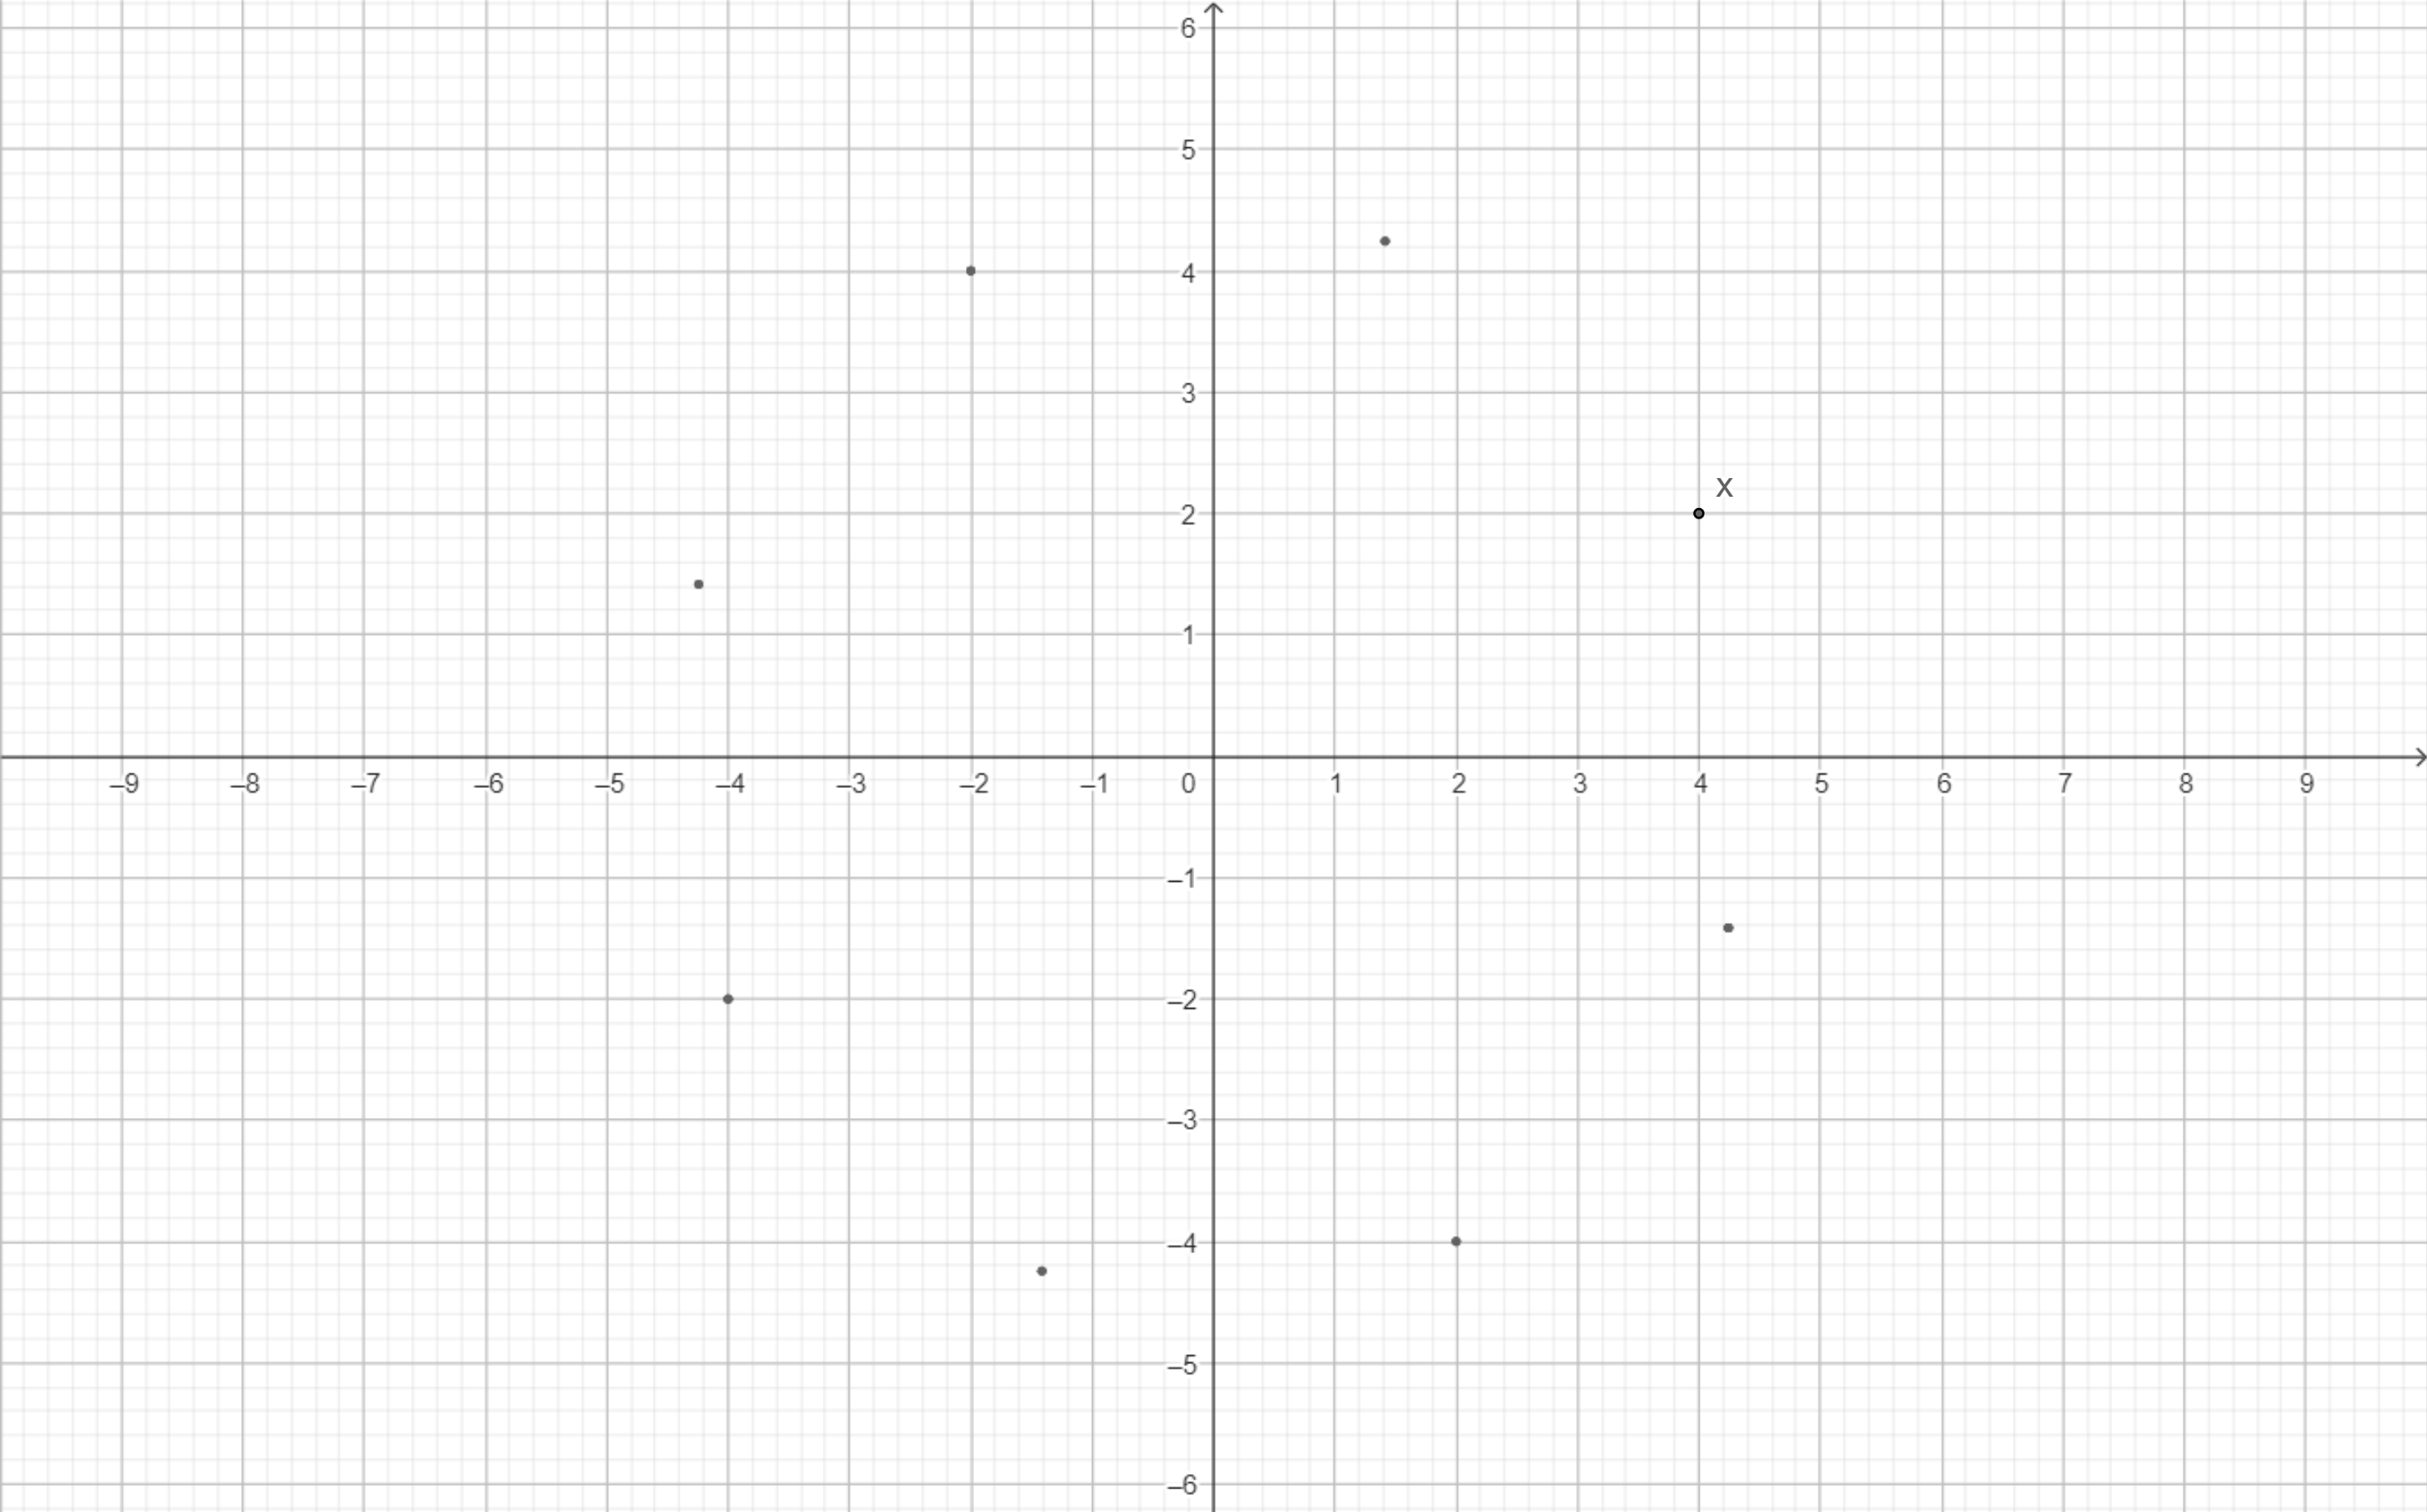
\includegraphics[width=0.5\textwidth]{4.2.png}
\end{figure} \\
С каждым шагом системы точка движется против часовой стрелки.\\[3em]
\subsubsection*{Пункт №3}
$$\begin{bmatrix}
    x_1(k) \\ x_2(k)
\end{bmatrix} = \begin{bmatrix}
    0 & -1 \\ 1 & 0
\end{bmatrix}^k\begin{bmatrix}
    4 \\ 2
\end{bmatrix} = \begin{bmatrix}
    \cos{\nicefrac{\pi k}{2}} & \sin{\nicefrac{\pi k}{2}} \\
    -\sin{\nicefrac{\pi k}{2}} & \cos{\nicefrac{\pi k}{2}}
\end{bmatrix}\begin{bmatrix}
    4 \\ 2
\end{bmatrix} = \begin{bmatrix}
    4\cos{\nicefrac{\pi k}{2}}+2\sin{\nicefrac{\pi k}{2}} \\
    2\cos{\nicefrac{\pi k}{2}}-4\sin{\nicefrac{\pi k}{2}}
\end{bmatrix}$$
\begin{figure}[h]
    \centering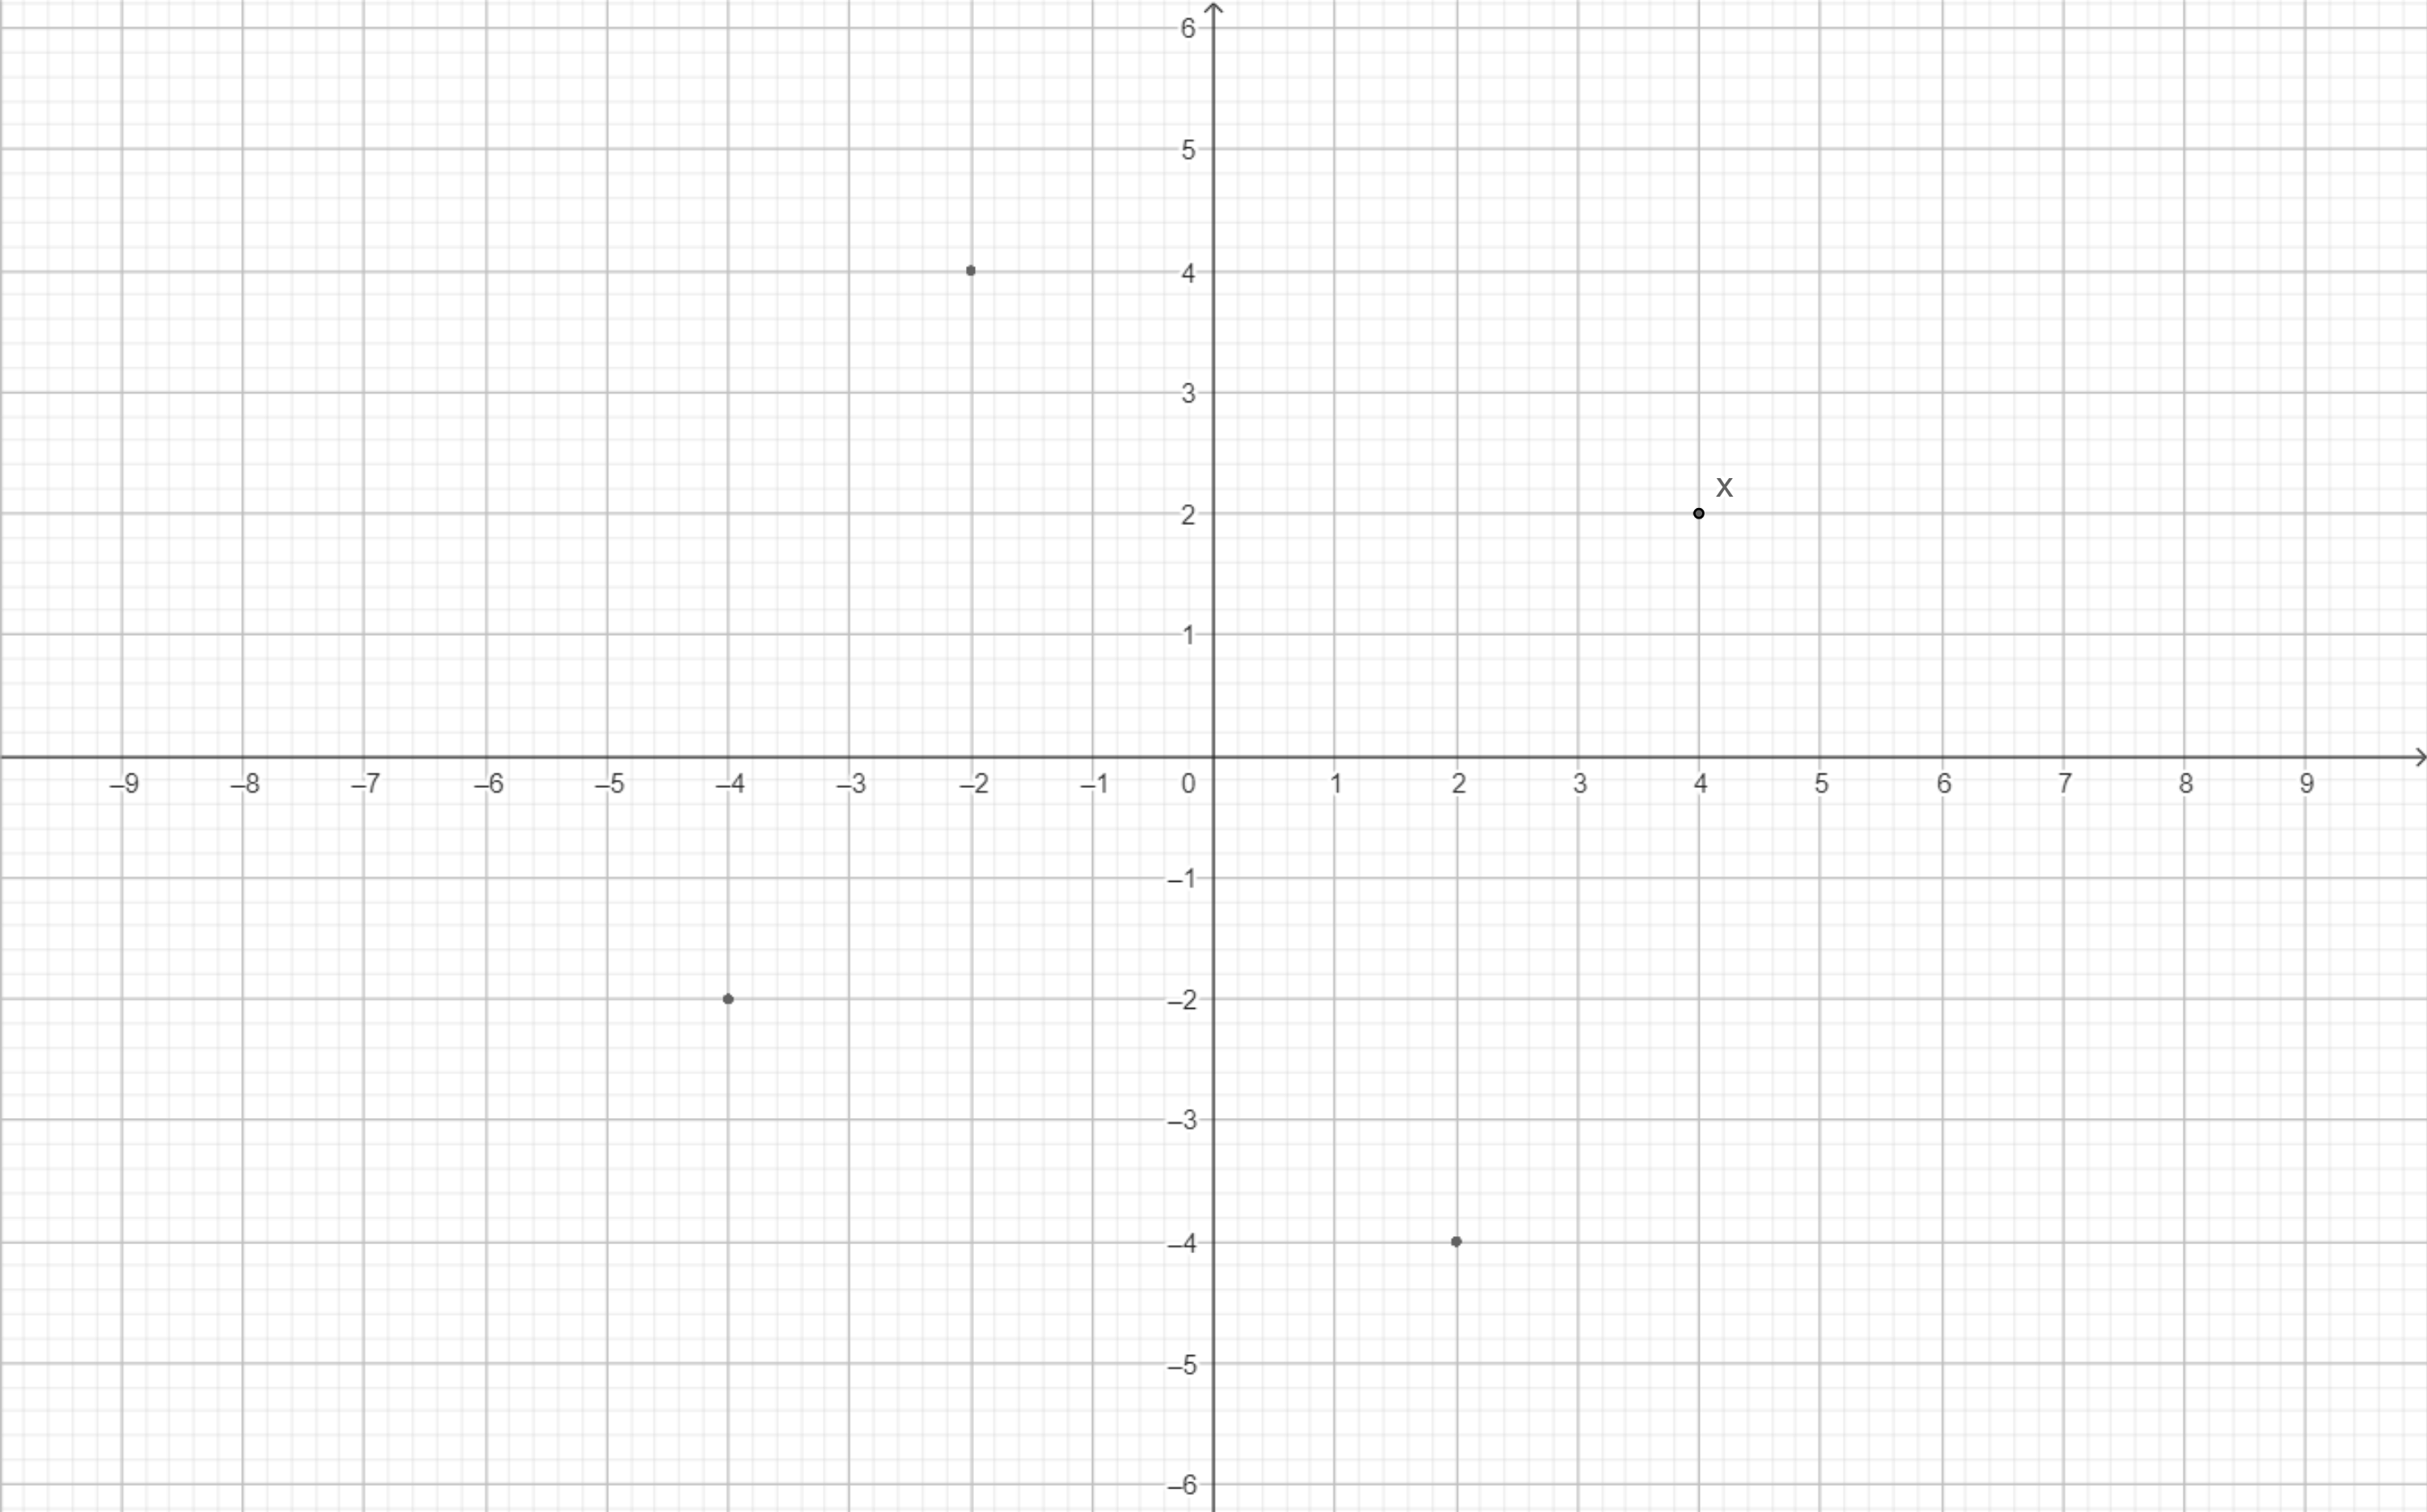
\includegraphics[width=0.5\textwidth]{4.3.png}
\end{figure} \\
С каждым шагом системы точка движется по часовой стрелке.
\pagebreak
\subsubsection*{Пункт №4}
$$\begin{bmatrix}
    x_1(k) \\ x_2(k)
\end{bmatrix} = \begin{bmatrix}
    \sqrt{2} & -\sqrt{2} \\ \nicefrac{\sqrt{2}}{2} & 0
\end{bmatrix}^k\begin{bmatrix}
    4 \\ 2
\end{bmatrix} = \begin{bmatrix}
    \cos{\nicefrac{\pi k}{4}} & \sin{\nicefrac{\pi k}{4}} \\
    -\sin{\nicefrac{\pi k}{4}} & \cos{\nicefrac{\pi k}{4}}
\end{bmatrix}\begin{bmatrix}
    4 \\ 2
\end{bmatrix} = \begin{bmatrix}
    4\cos{\nicefrac{\pi k}{4}}+2\sin{\nicefrac{\pi k}{4}} \\
    2\cos{\nicefrac{\pi k}{4}}-4\sin{\nicefrac{\pi k}{4}}
\end{bmatrix}$$
\begin{figure}[h]
    \centering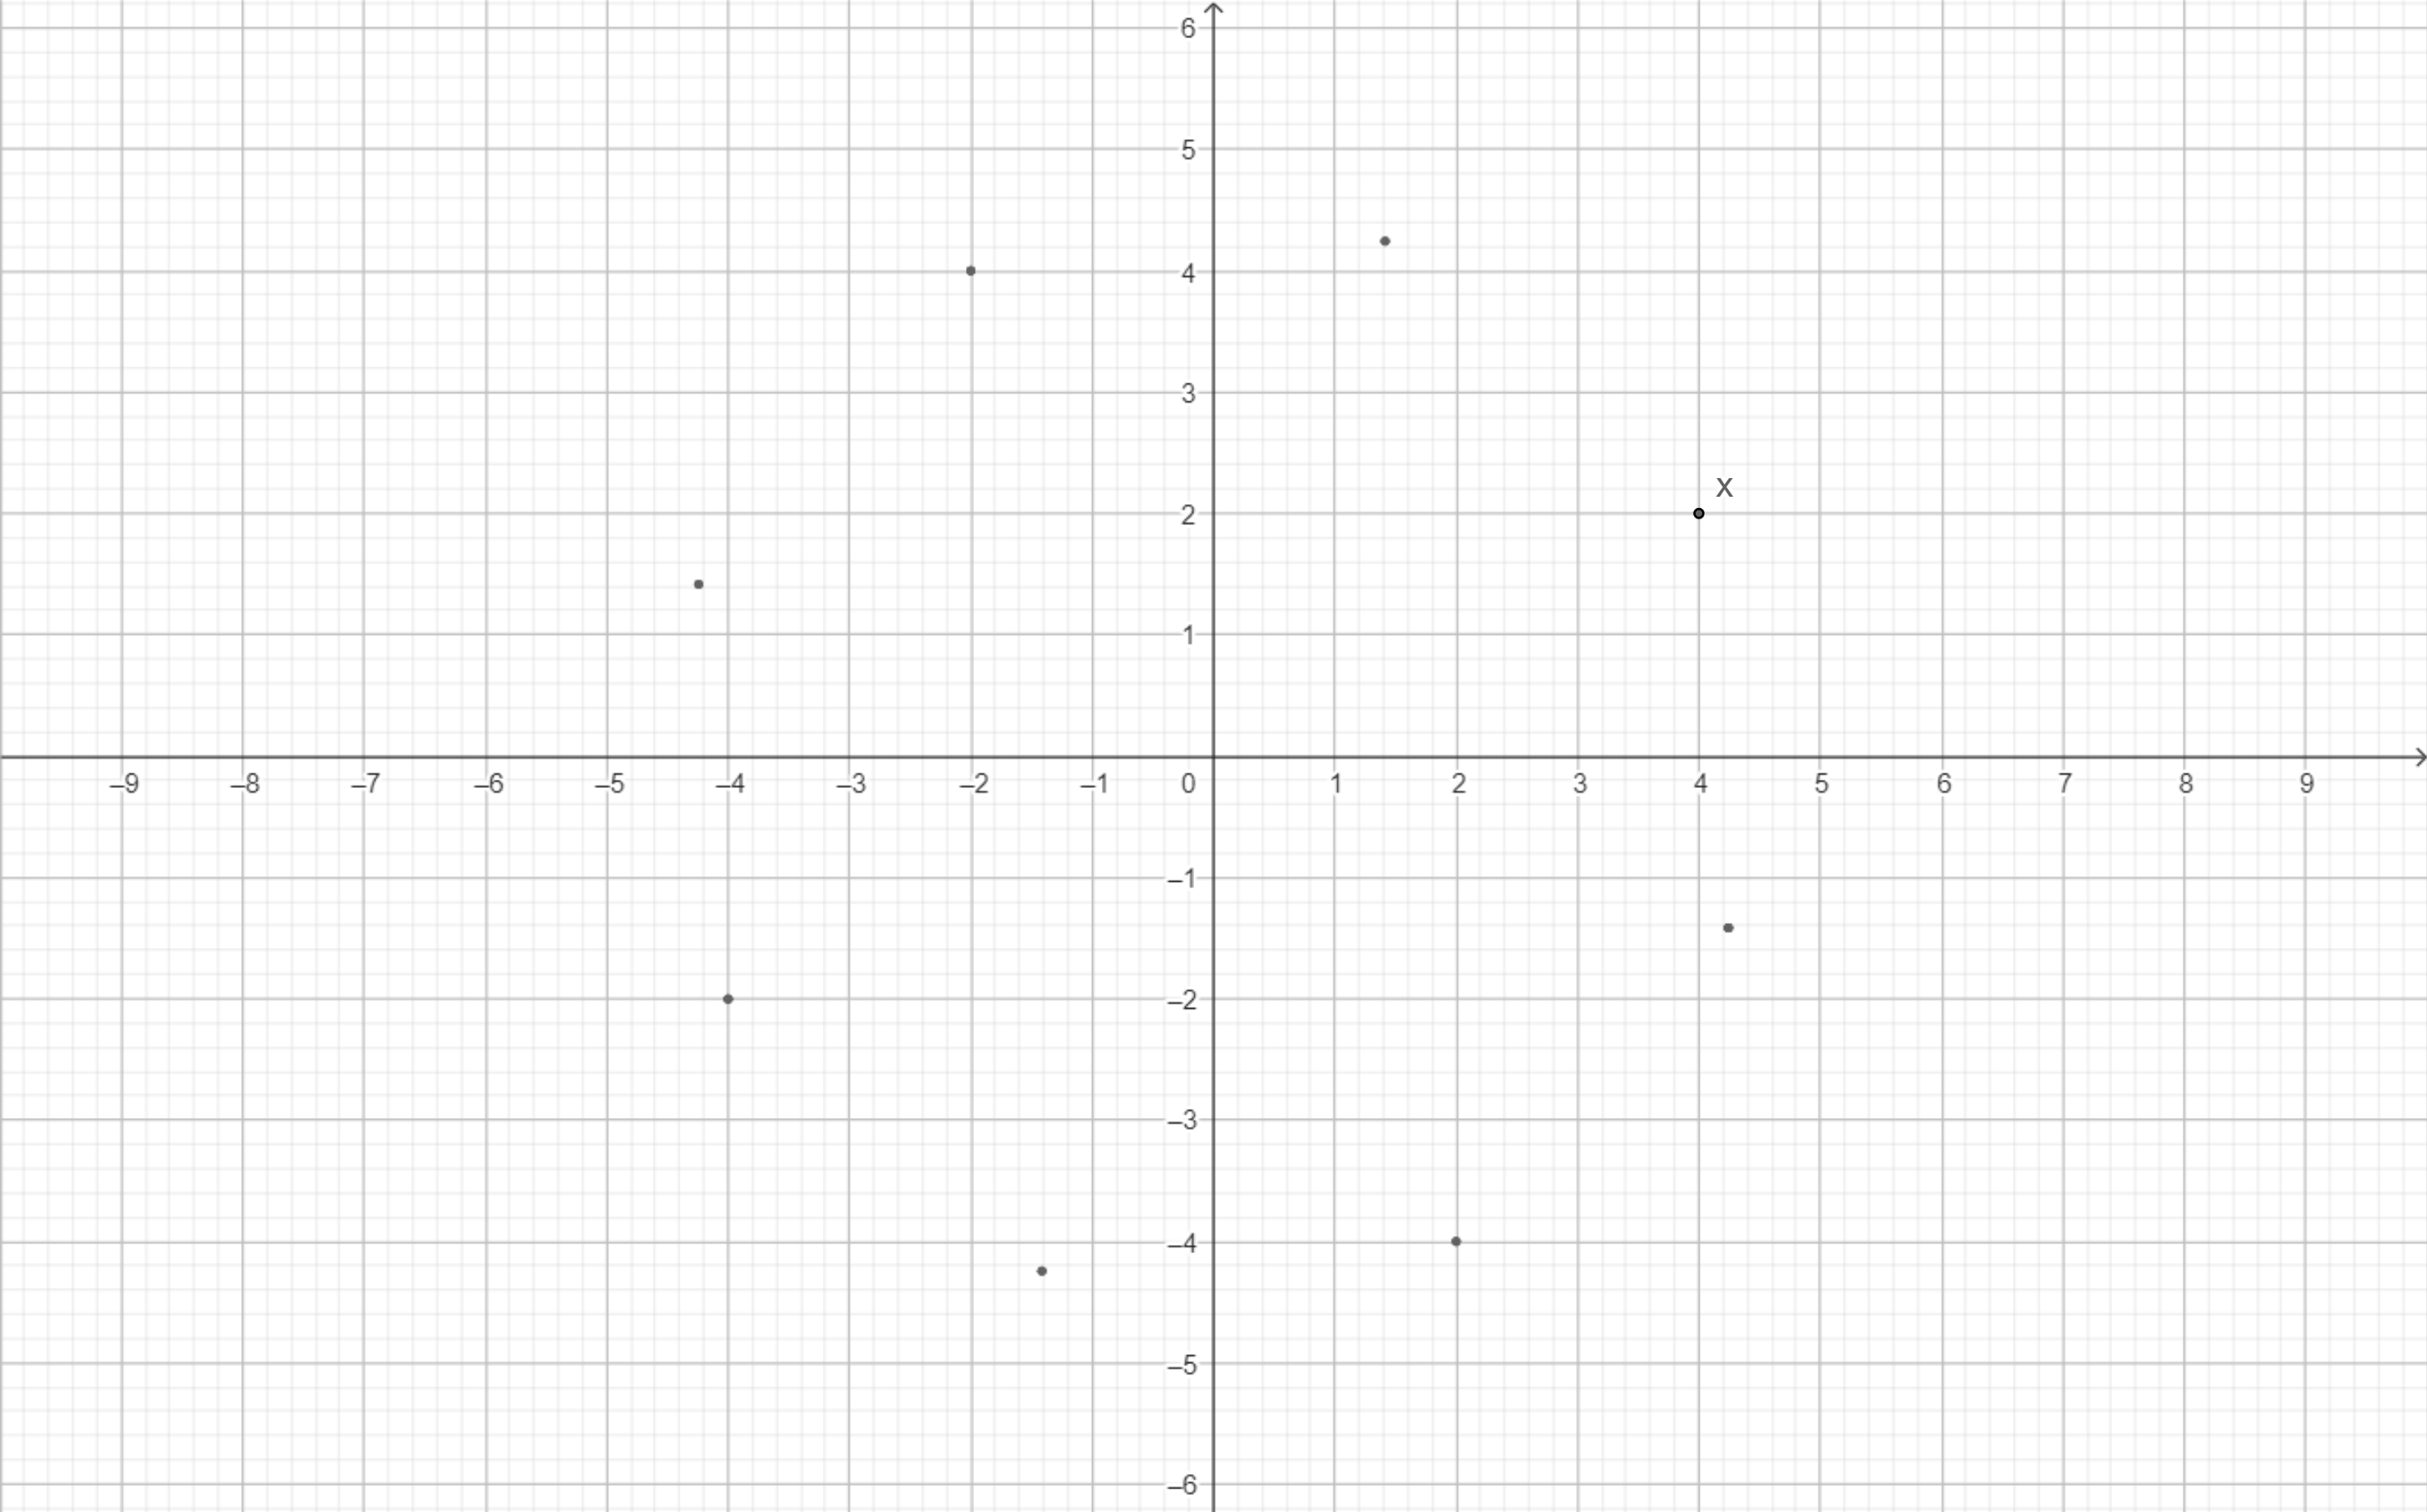
\includegraphics[width=0.5\textwidth]{4.2.png}
\end{figure} \\
Как и в предыдущем пункте, с каждым шагом системы точка движется по часовой стрелке.\\[3em]
\subsubsection*{Пункт №5}
$$\begin{bmatrix}
    x_1(k) \\ x_2(k)
\end{bmatrix} = \begin{bmatrix}
    \nicefrac{5}{2} & \nicefrac{-1}{2} \\
    \nicefrac{9}{2} & \nicefrac{-1}{2}
\end{bmatrix}^k\begin{bmatrix}
    4 \\ 2
\end{bmatrix} = \begin{bmatrix}
    \nicefrac{3k+2}{2} & \nicefrac{-k}{2} \\ \nicefrac{9k}{2} & \nicefrac{-3k+2}{2}
\end{bmatrix}\begin{bmatrix}
    4 \\ 2
\end{bmatrix} = \begin{bmatrix}
    5k+4 \\ 15k+12
\end{bmatrix}$$
\begin{figure}[h]
    \centering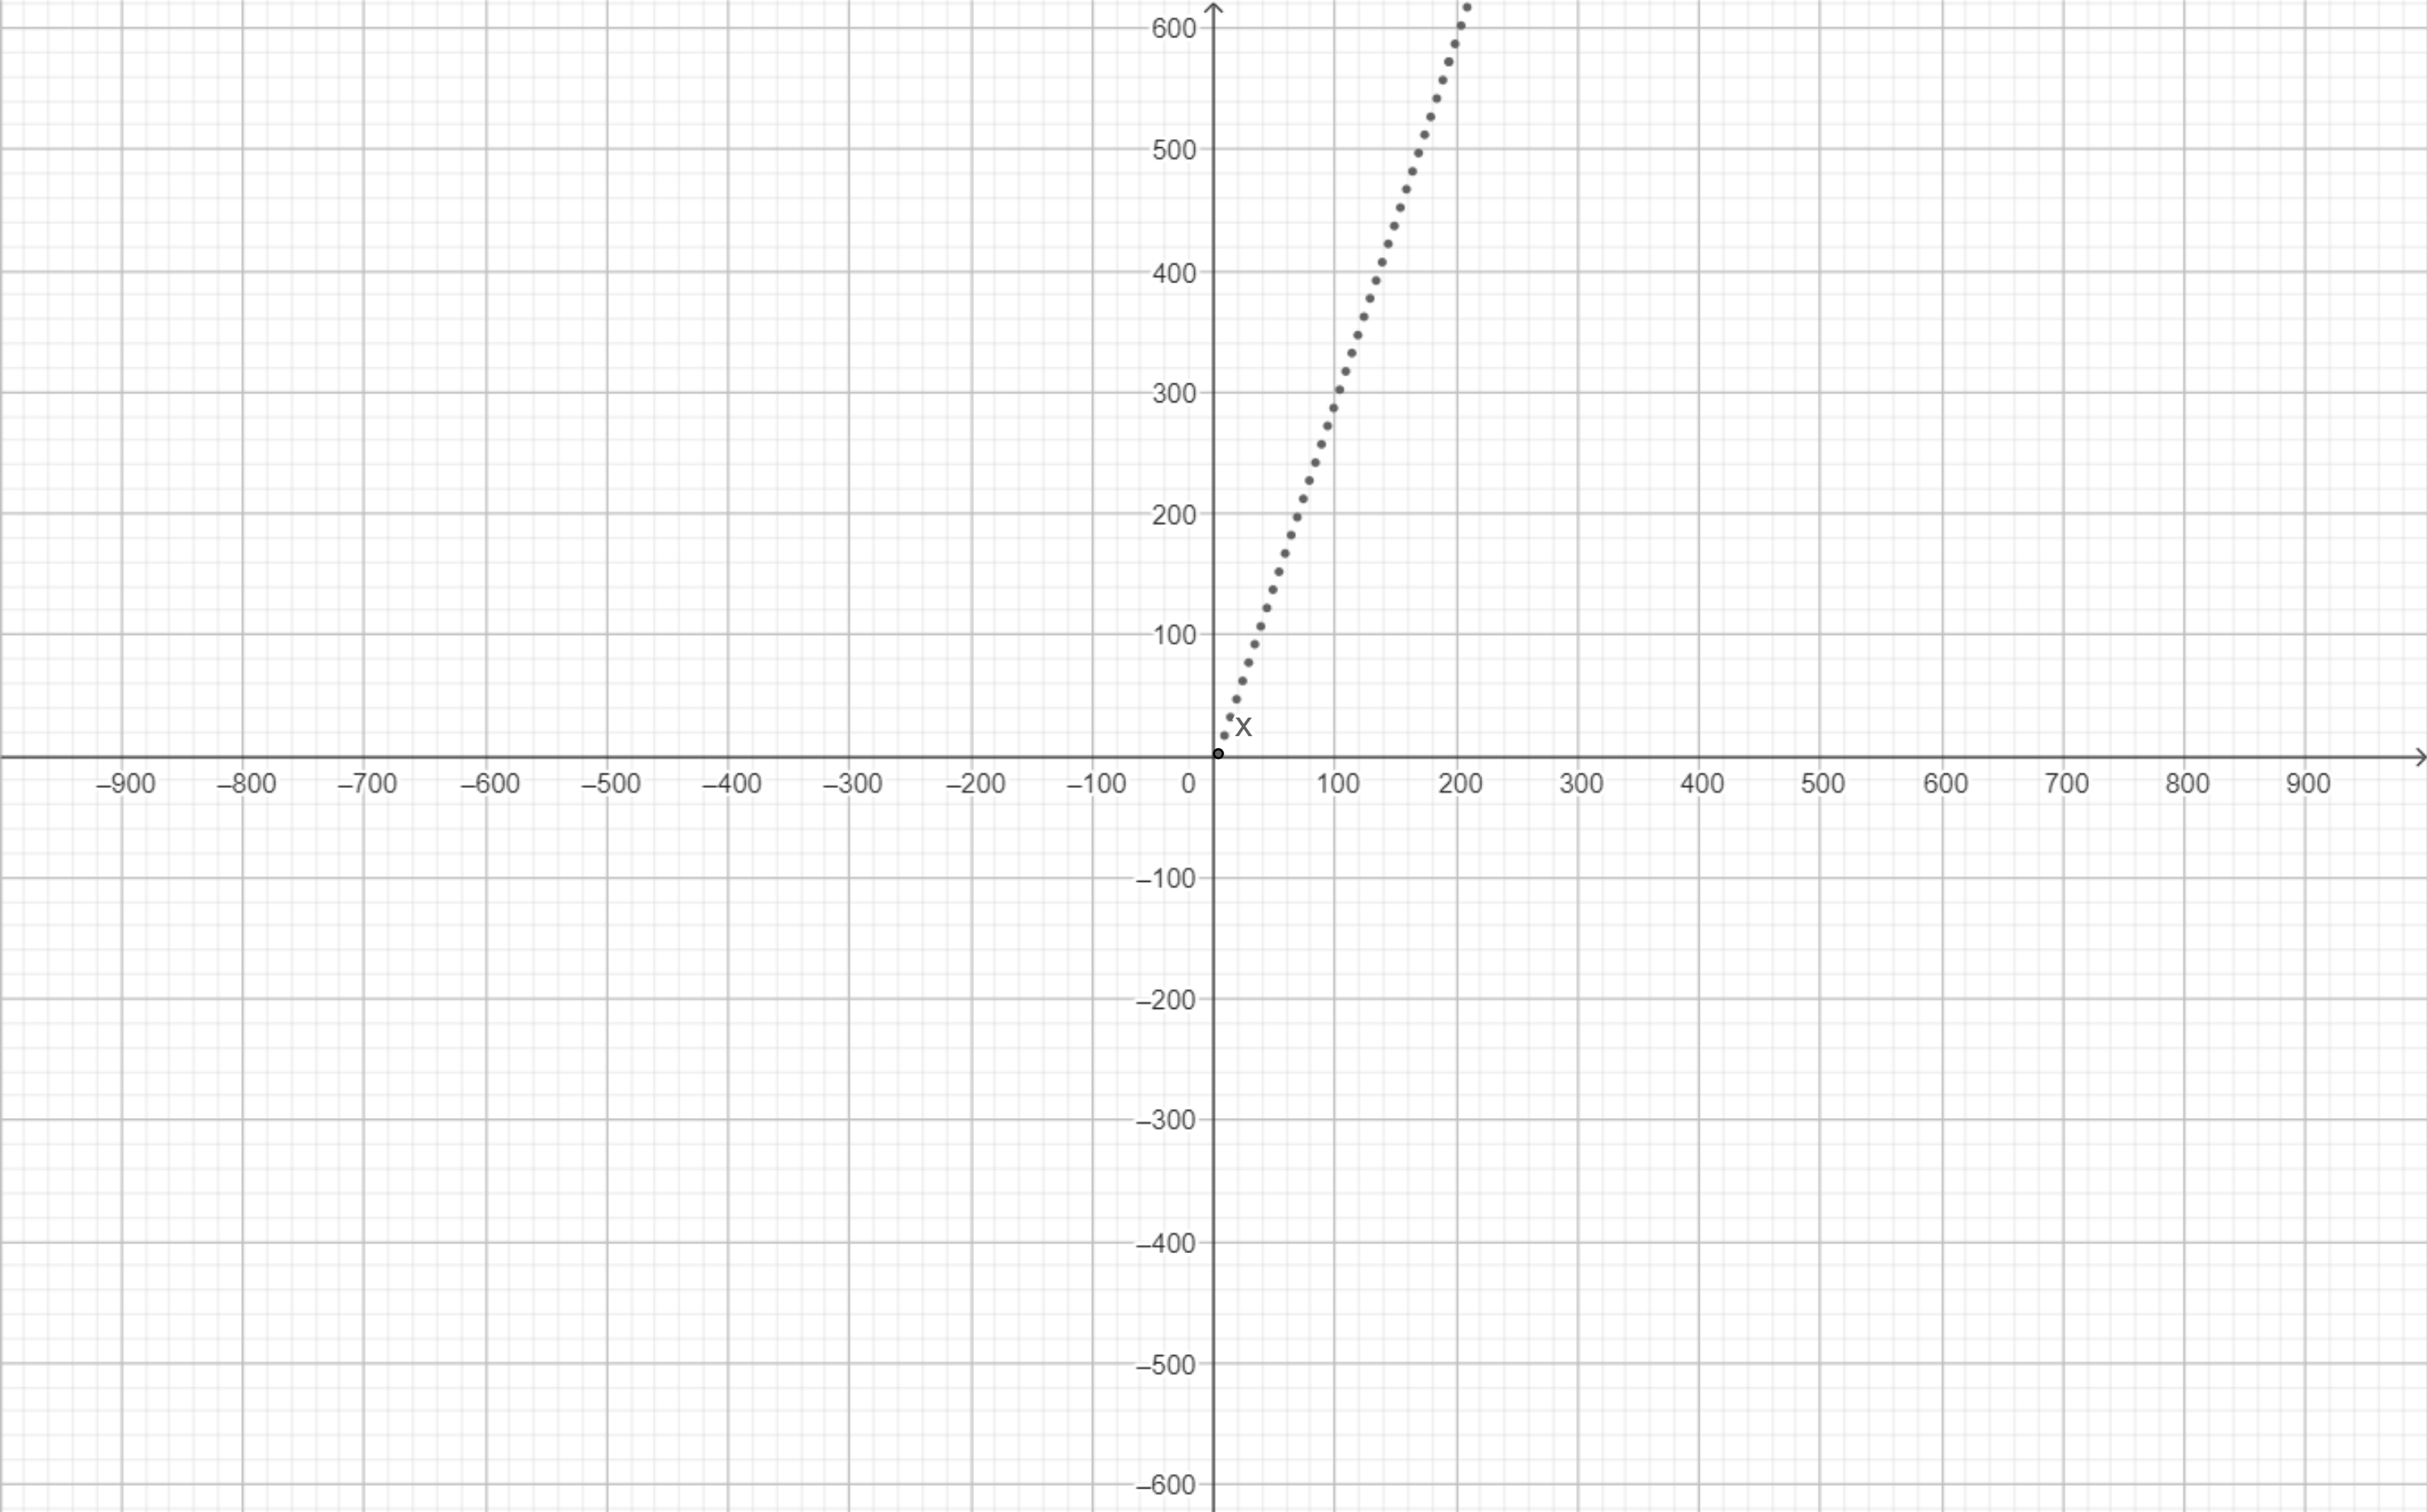
\includegraphics[width=0.5\textwidth]{4.5.png}
\end{figure} \\[1em]
\textit{К сожалению, студент был голодний, поэтому он бахнув пельменів --- мы решили сделать за него 6-12 пункты\ldots}\\[0.5em]
На самом деле весь секрет в том, что если выполняется условие $|\lambda| < 1$ для собственных чисел матрицы дискретной системы, то тогда можно говорить об асимптотической устойчивости. Мы увидели в пунктах №1,5, что система оказывается неустойчивой при $\lambda = \pm1$ --- так получилось потому, что для матрицы отсутствовал базис собственных векторов, в противном же случае система была бы не асимптотически устойчивой.\\[0.5em]
А что же с комплексными числами? Если у матрицы системы имеется пара собственных чисел $\lambda = a\pm bi$, то система асимптотически устойчива, когда $\sqrt{a^2+b^2}<1$. В случае, когда $\sqrt{a^2+b^2}=1$, система устойчива, но не асимптотически.\\[0.5em]
Интересно рассмотреть и последний случай. Даже при наличии жорданового разложения, мы получим $J^k = \left[\begin{smallmatrix}
    0^k & 0^{k-1}k \\ 0 & 0^k
\end{smallmatrix}\right]$, поэтому на следующем же шаге все точки системы обращаются в ноль.
\subsection*{\centering Задание №5. Осциллятор???}
\textit{Помнится, студент бахнув пельменів --- так вот его разморило, он наелся и спит\ldots Мы пытались его разбудить, но безуспешно\ldots}
\end{document}